\chapter{Implementation}


% 	Explain Implementation details :
% 	Experimental setup
% 	Scenarios, Testing, Results, Analysis, Graphs, Comparison with earlier work
	
% 	Also add Screen shots and Code sample here.
	
% 	Write in detail about the Testing Tools used (i.e. it's purpose in this project etc.) and Test plans executed and snapshots of the testing performed.
\section{Screen shots}
\begin{figure}[!h]
	\centering
	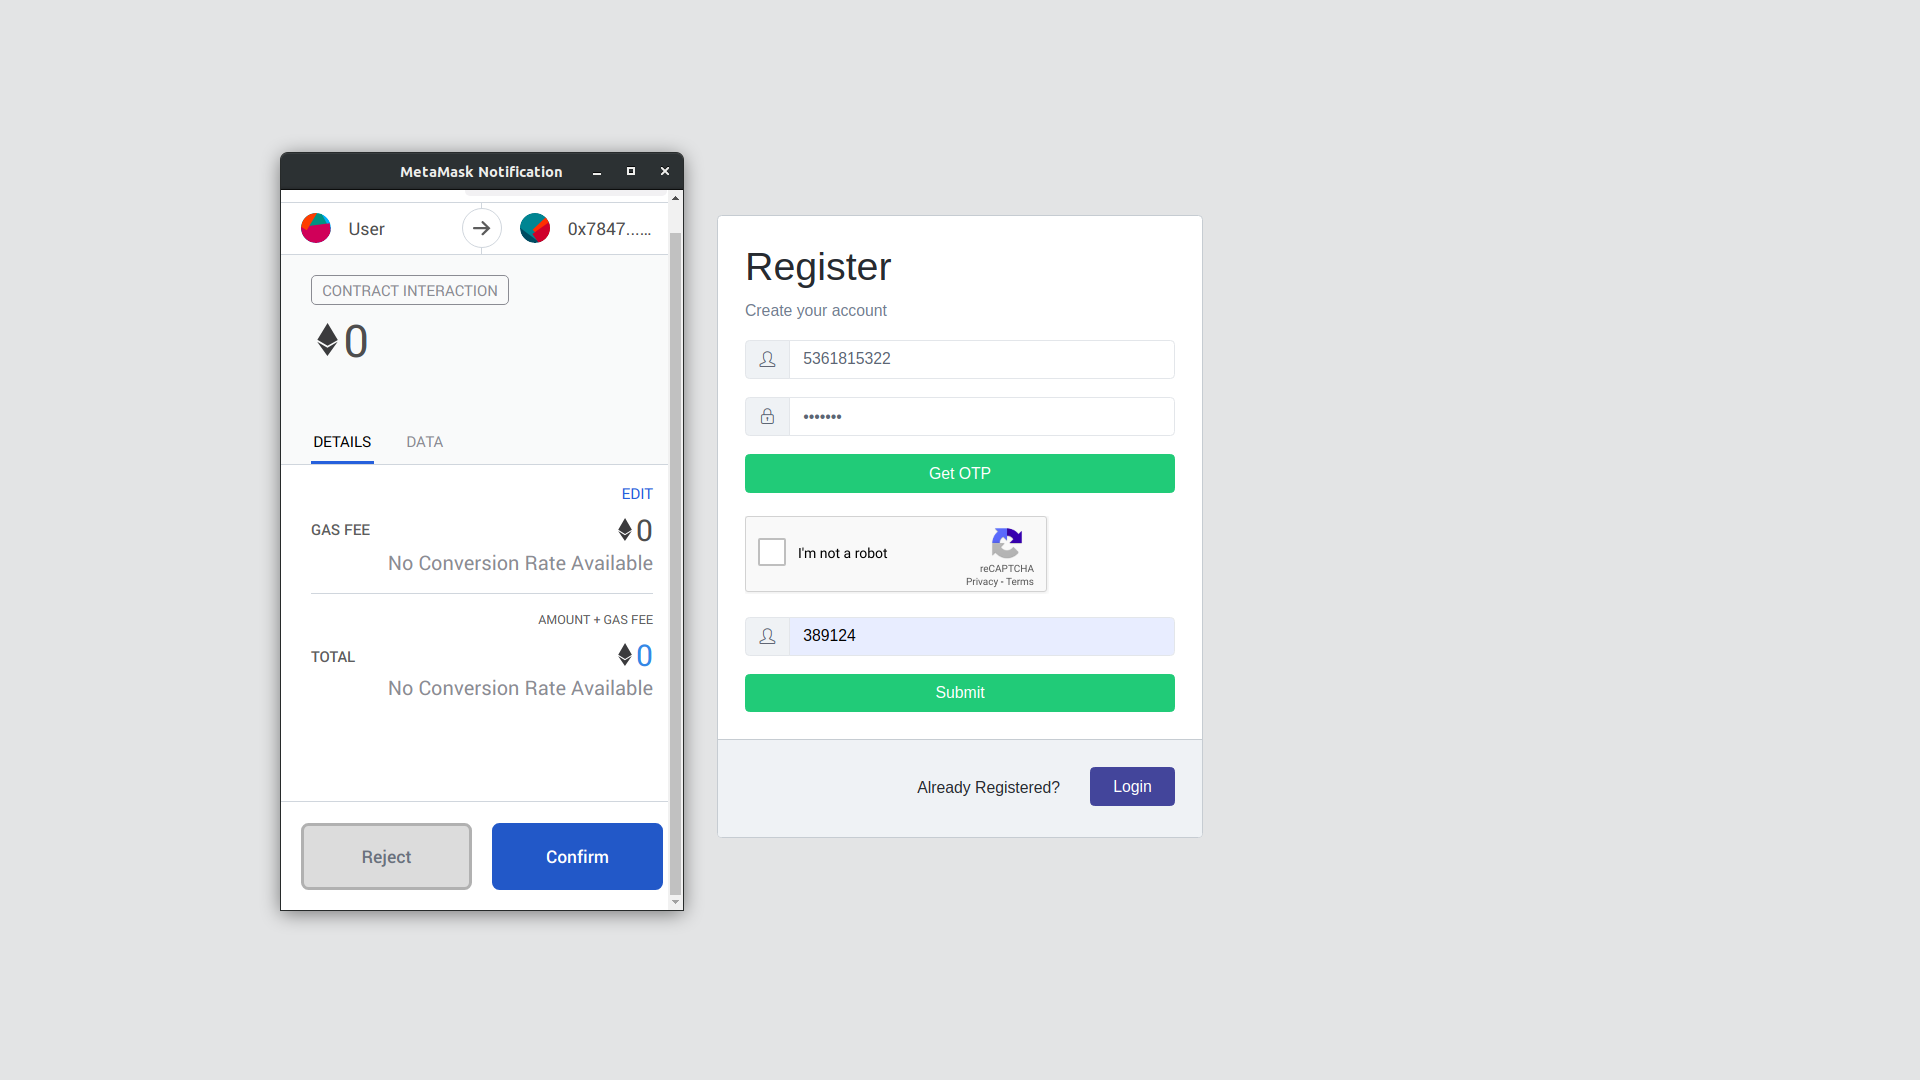
\includegraphics[width=\linewidth]{Images/User/UserRegistration.png}
	\caption{User Registration}
	%\label{fig:universe}
\end{figure}
\begin{figure}[!b]
	\centering
	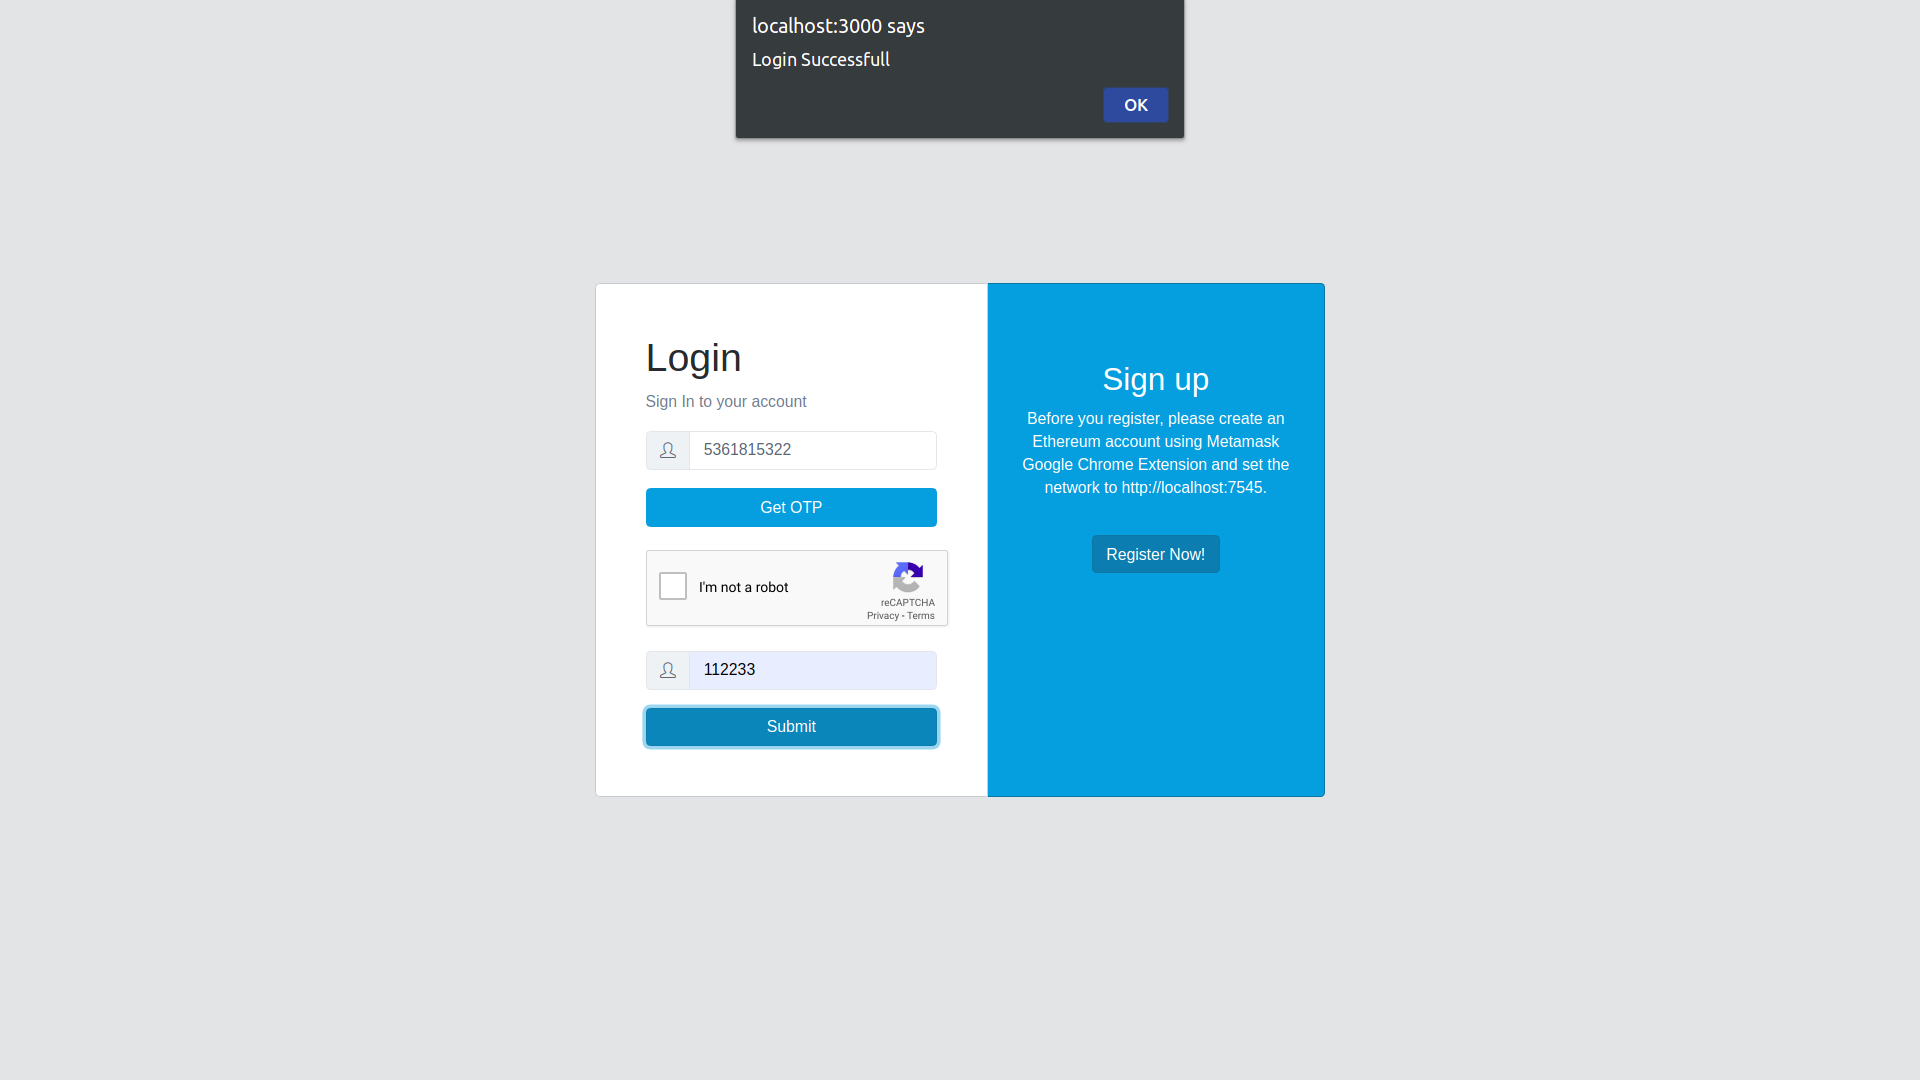
\includegraphics[width=\linewidth]{Images/User/UserLogin.png}
	\caption{User Login}
	%\label{fig:universe}
\end{figure}

\begin{figure}[!h]
	\centering
	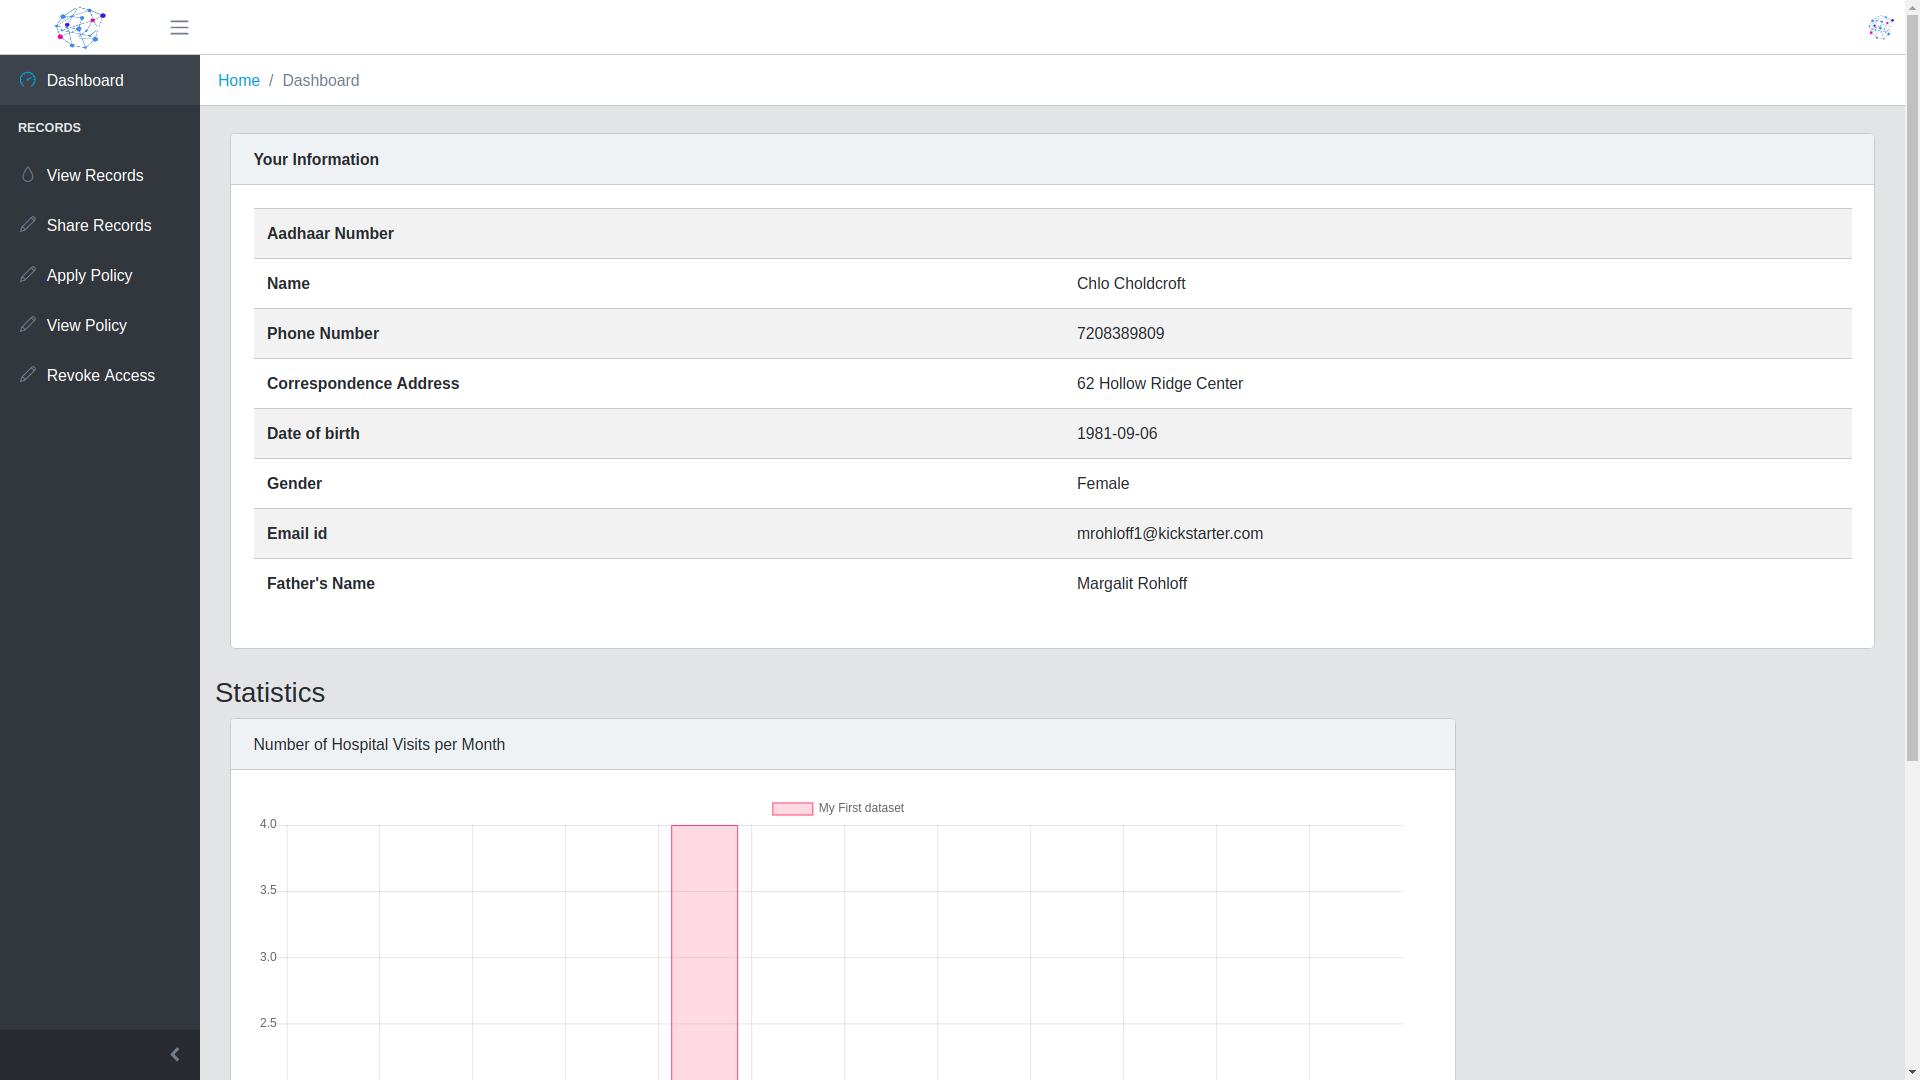
\includegraphics[width=\linewidth]{Images/User/UserDashboard.png}
	\caption{User Dashboard}
	%\label{fig:universe}
\end{figure}
\begin{figure}[!b]
	\centering
	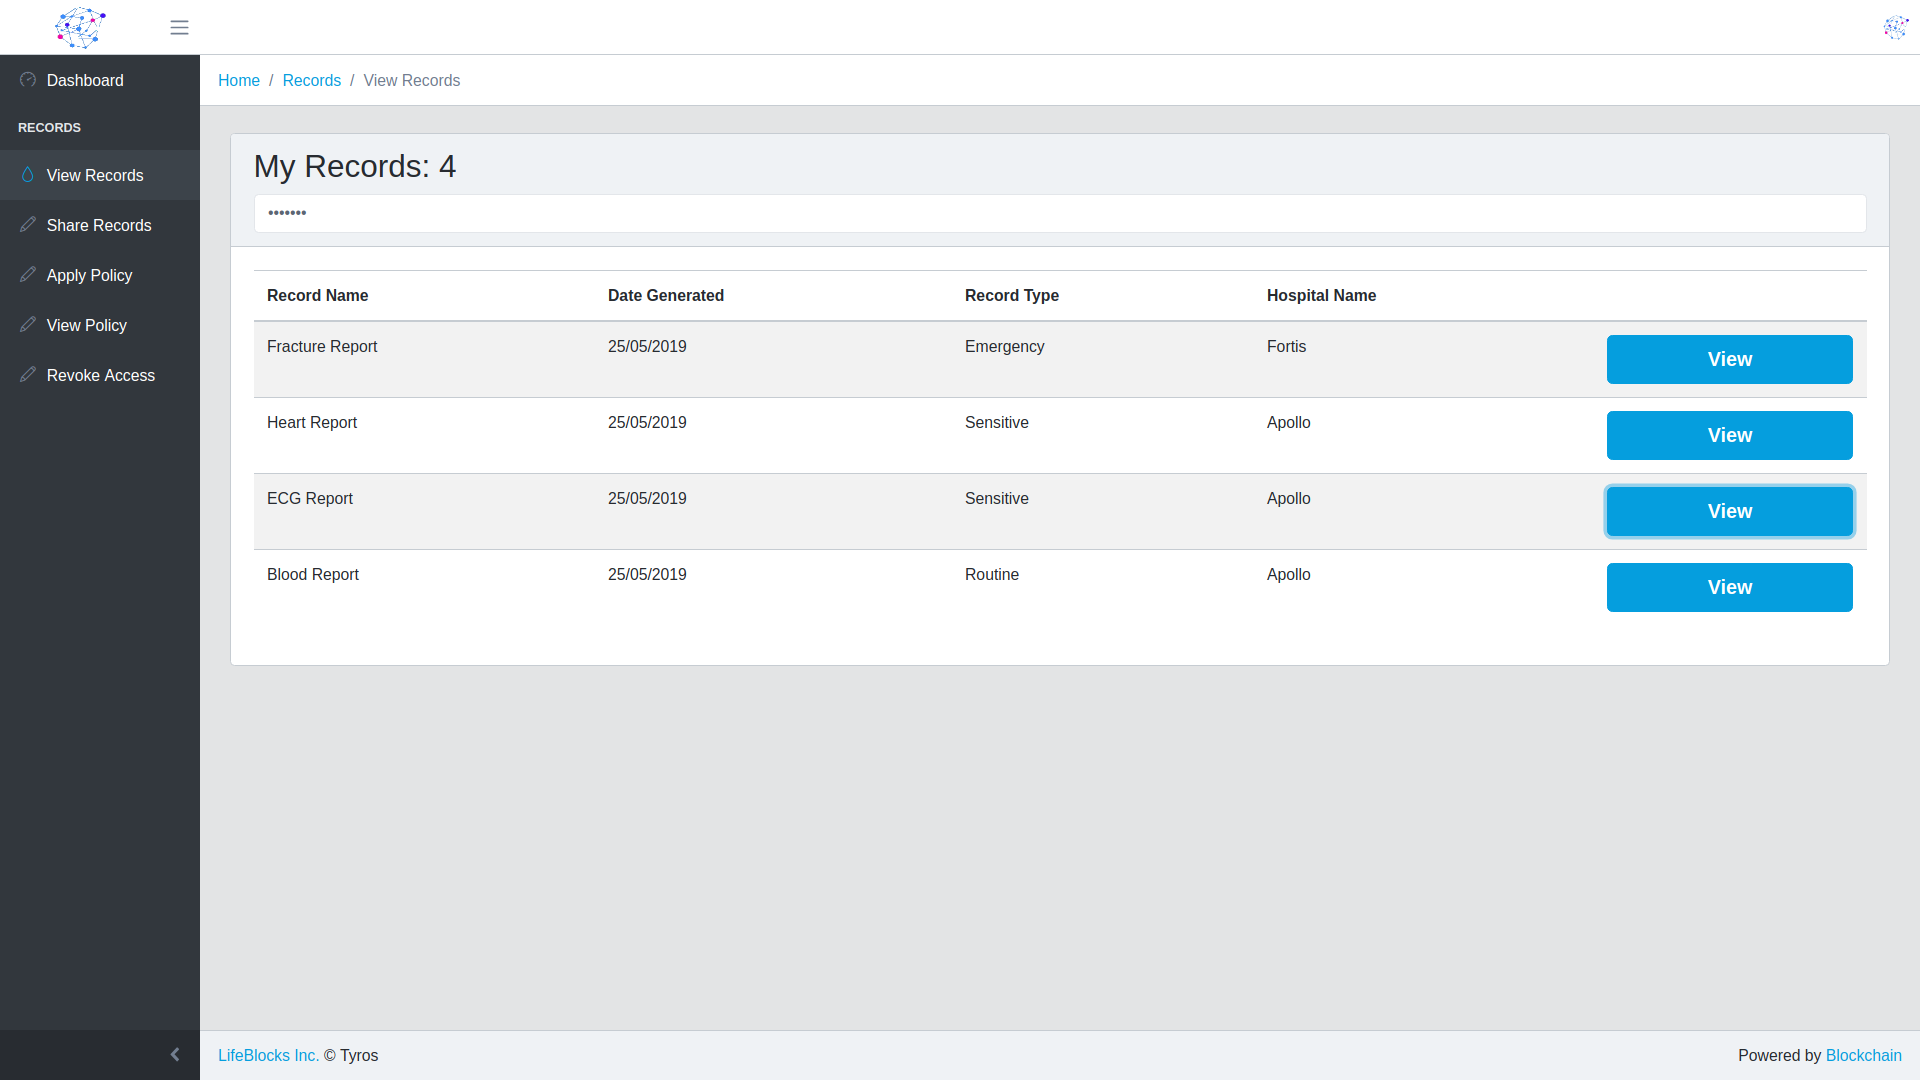
\includegraphics[width=\linewidth]{Images/User/UserViewRecord1.png}
	\caption{ User View Record (a)}
	%\label{fig:universe}
\end{figure}

\begin{figure}[!h]
	\centering
	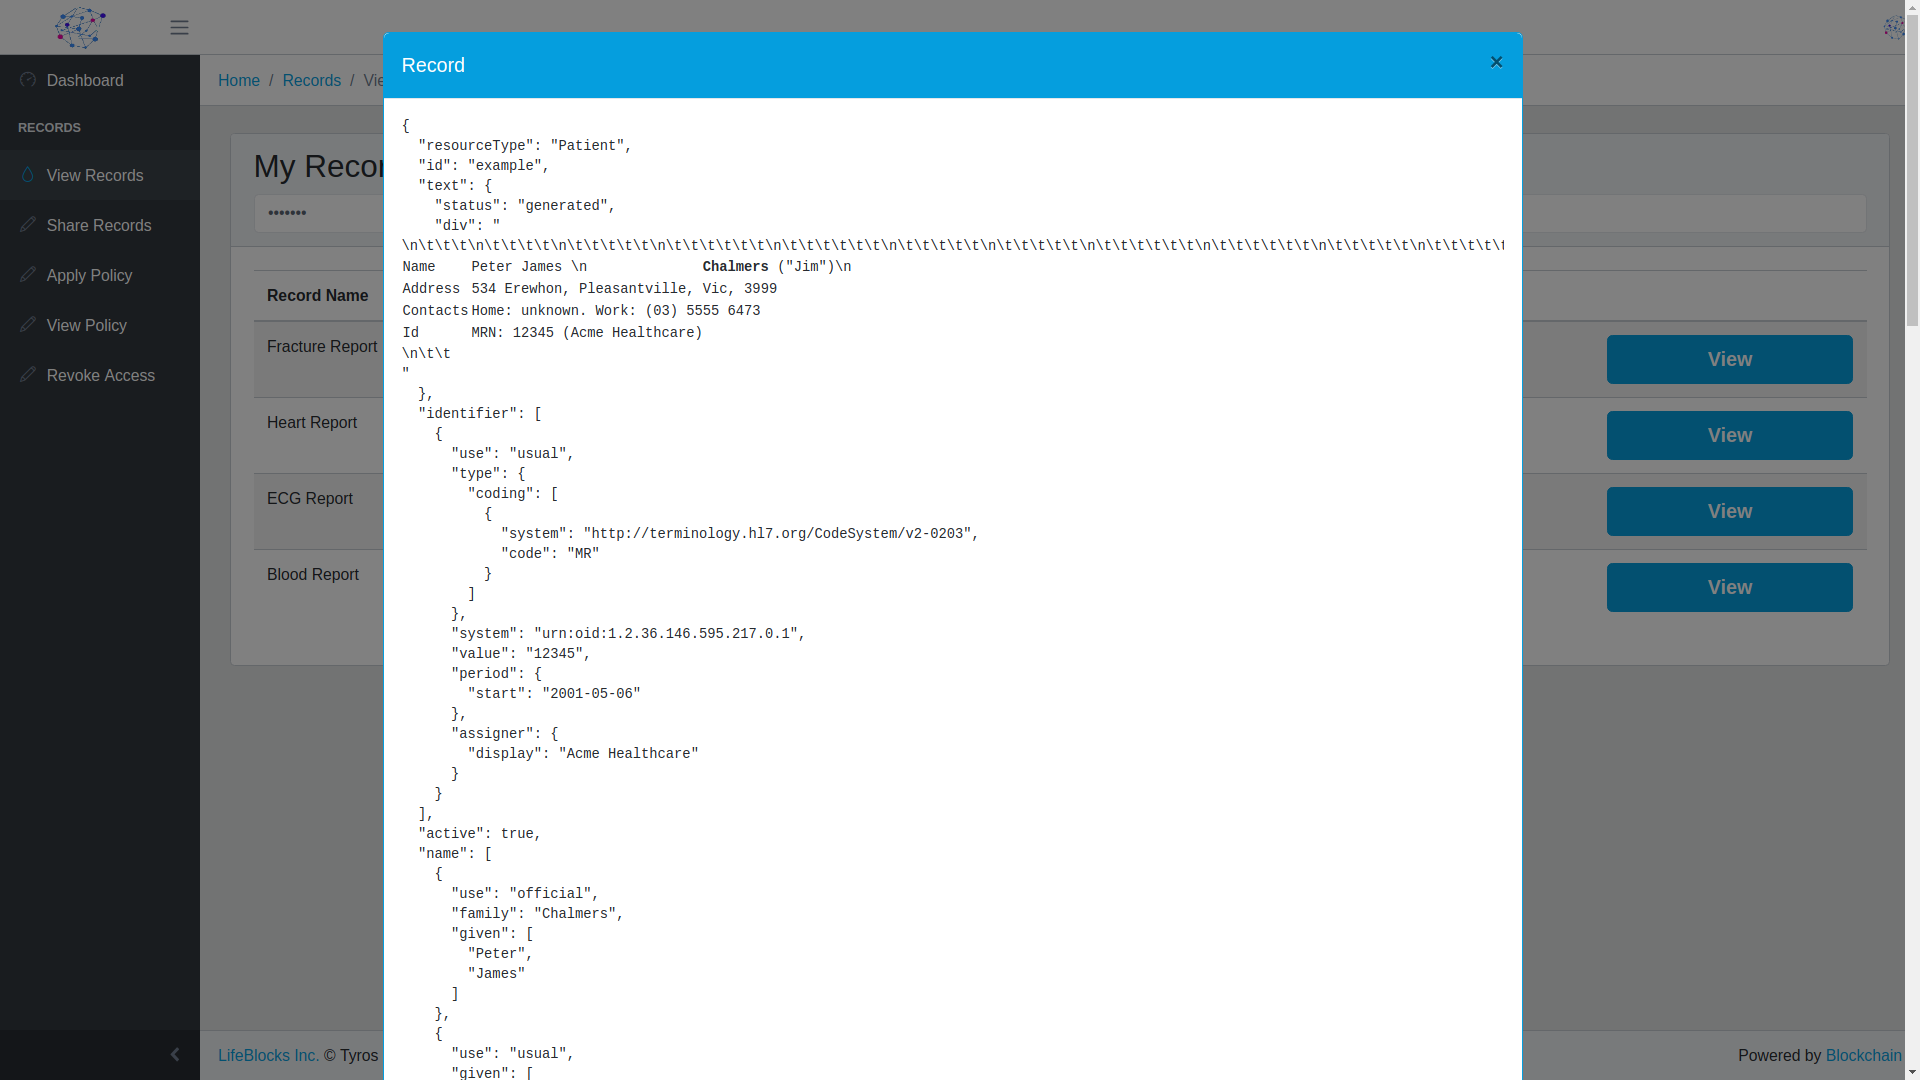
\includegraphics[width=\linewidth]{Images/User/UserViewRecord2.png}
	\caption{ User View Record (b)}
	%\label{fig:universe}
\end{figure}
\begin{figure}[!b]
	\centering
	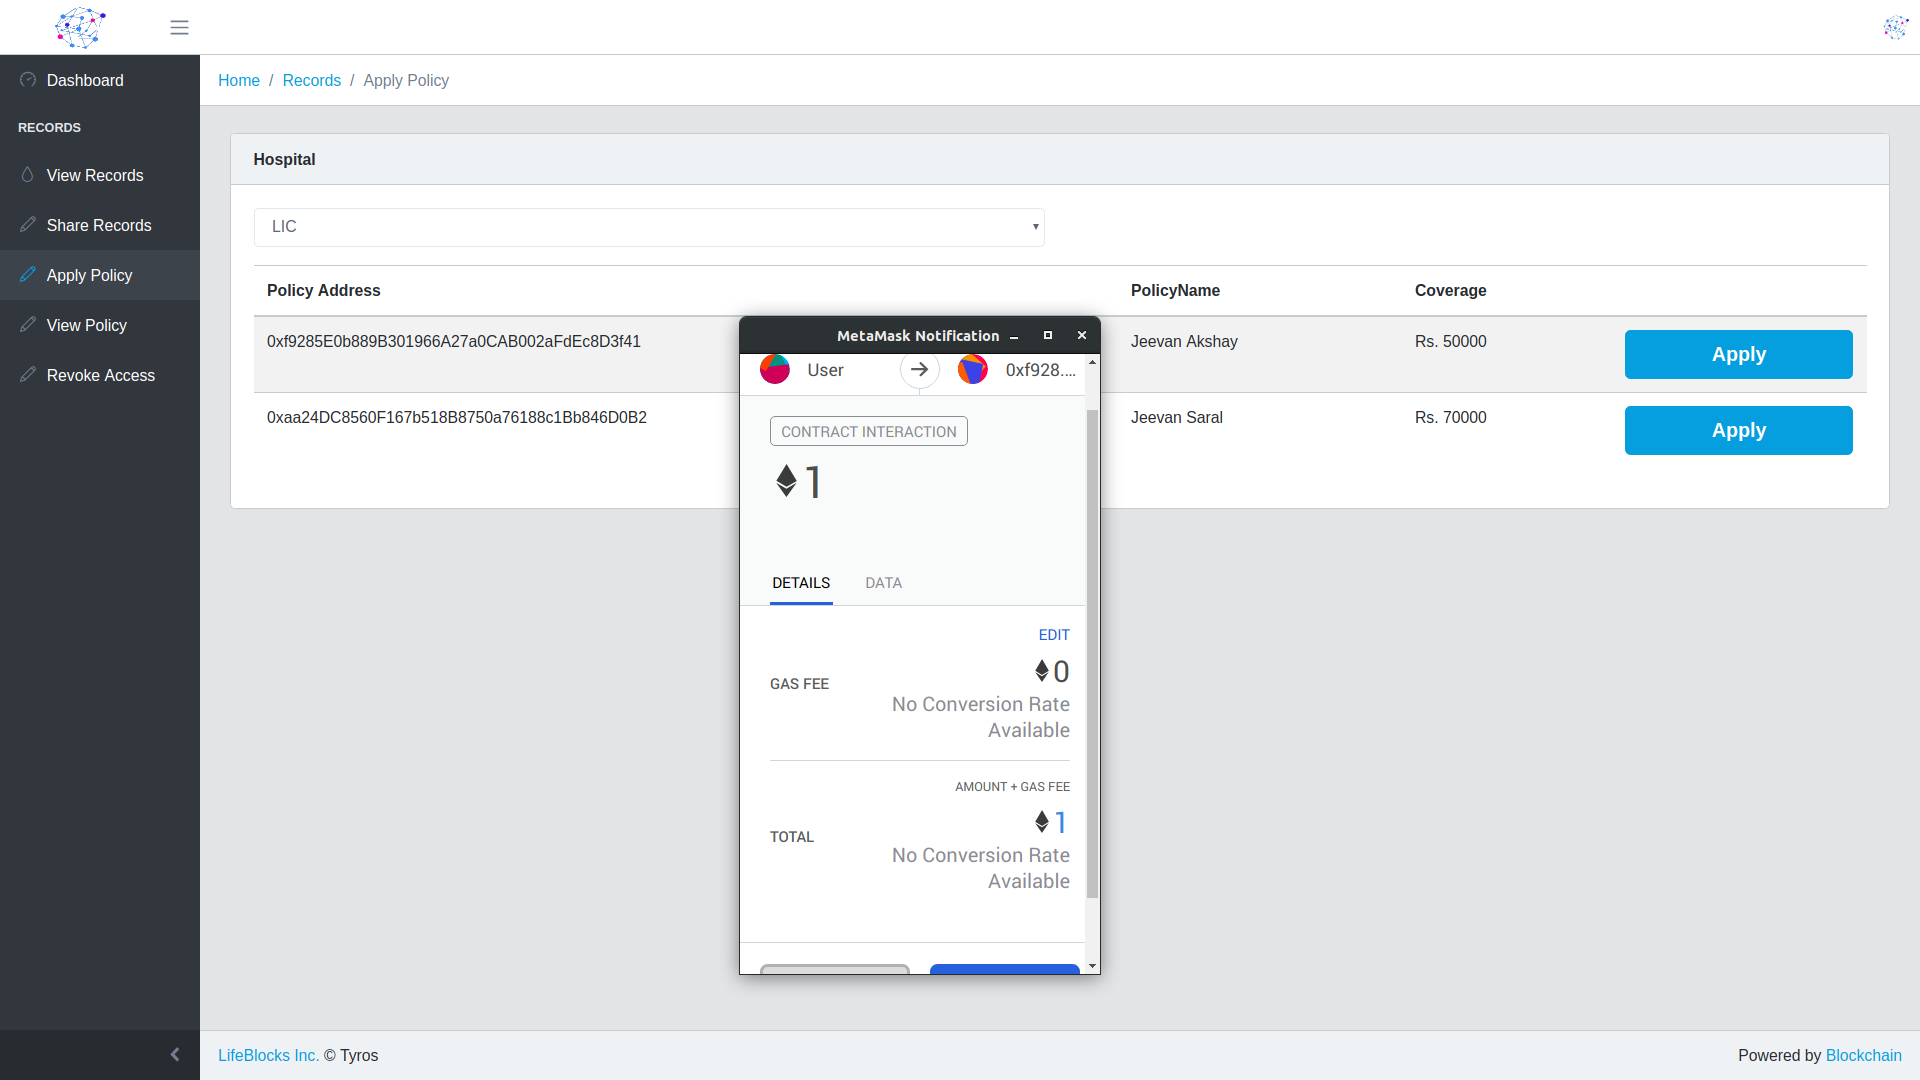
\includegraphics[width=\linewidth]{Images/User/UserApplyPolicy.png}
	\caption{ User Apply Policy}
	%\label{fig:universe}
\end{figure}

\begin{figure}[!b]
	\centering
	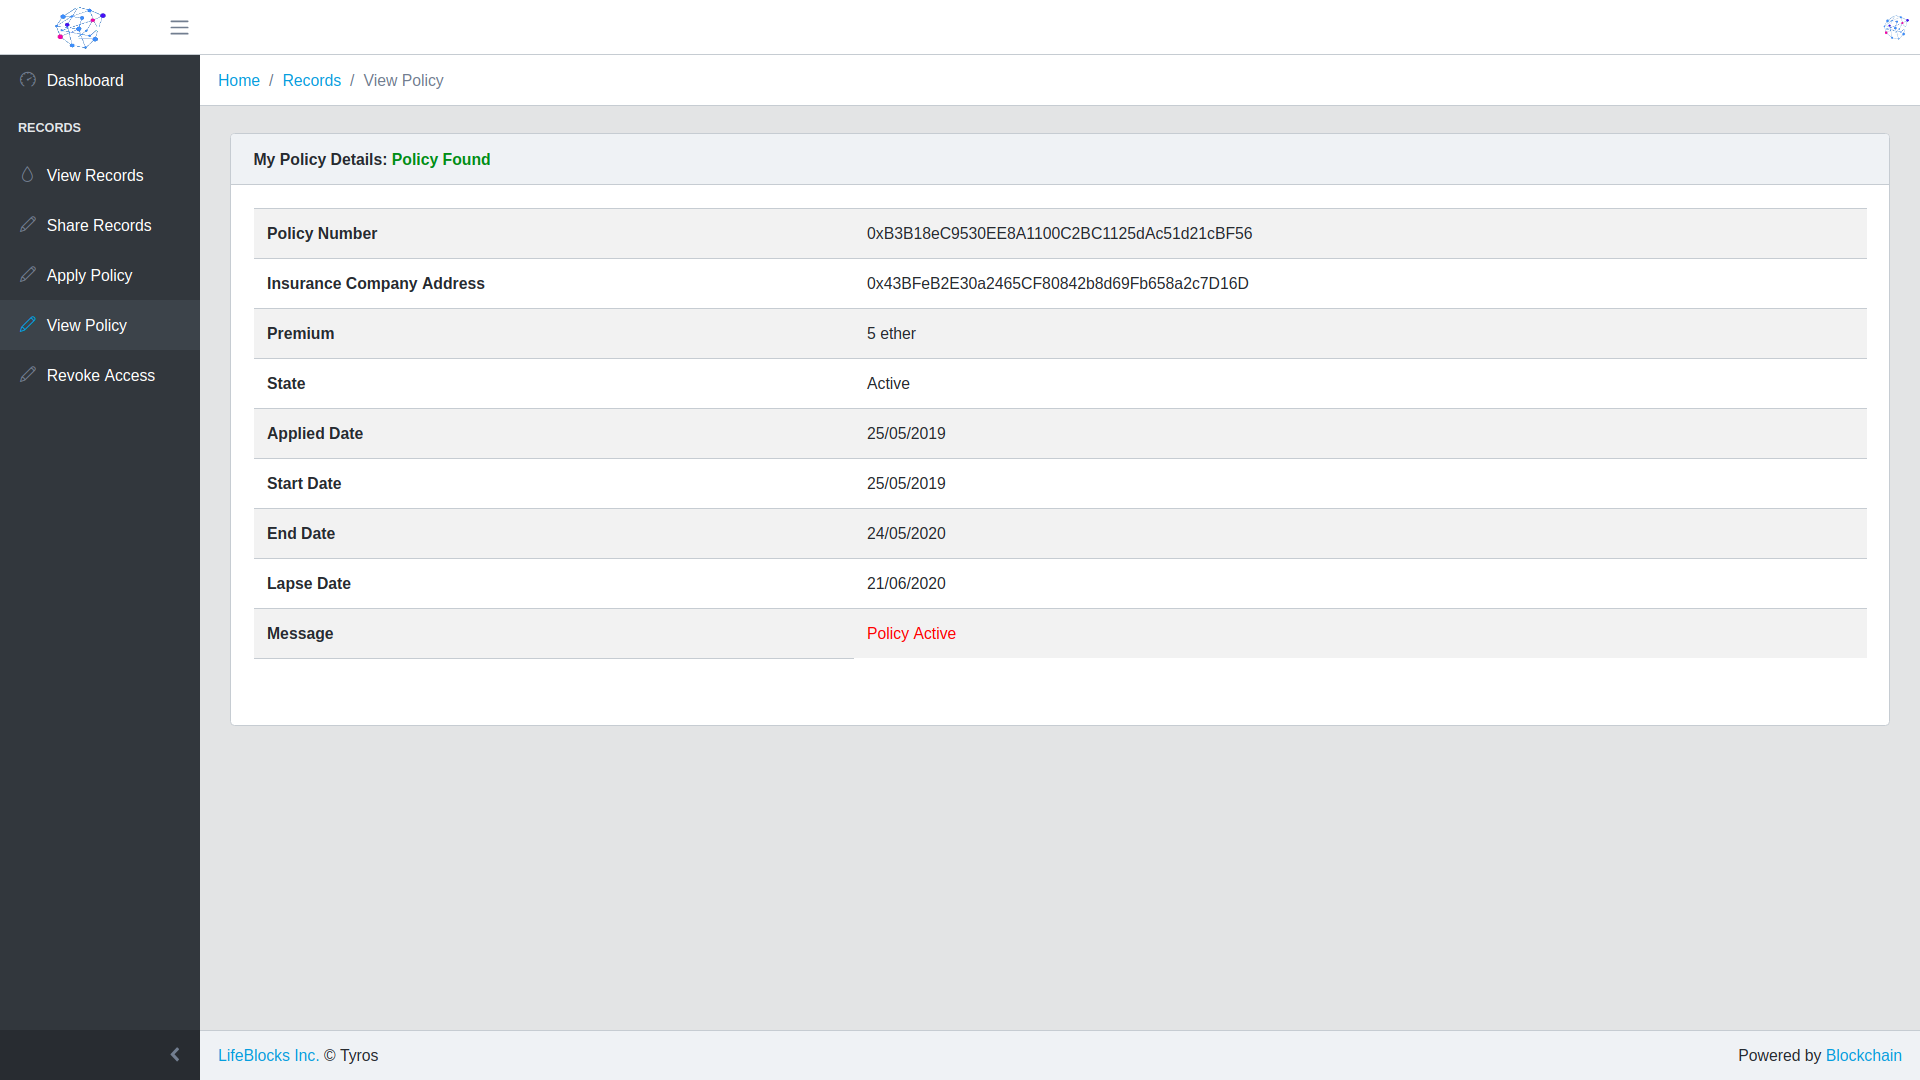
\includegraphics[width=\linewidth]{Images/User/UserViewPolicy.png}
	\caption{ User View Policy}
	%\label{fig:universe}
\end{figure}
\begin{figure}[!b]
	\centering
	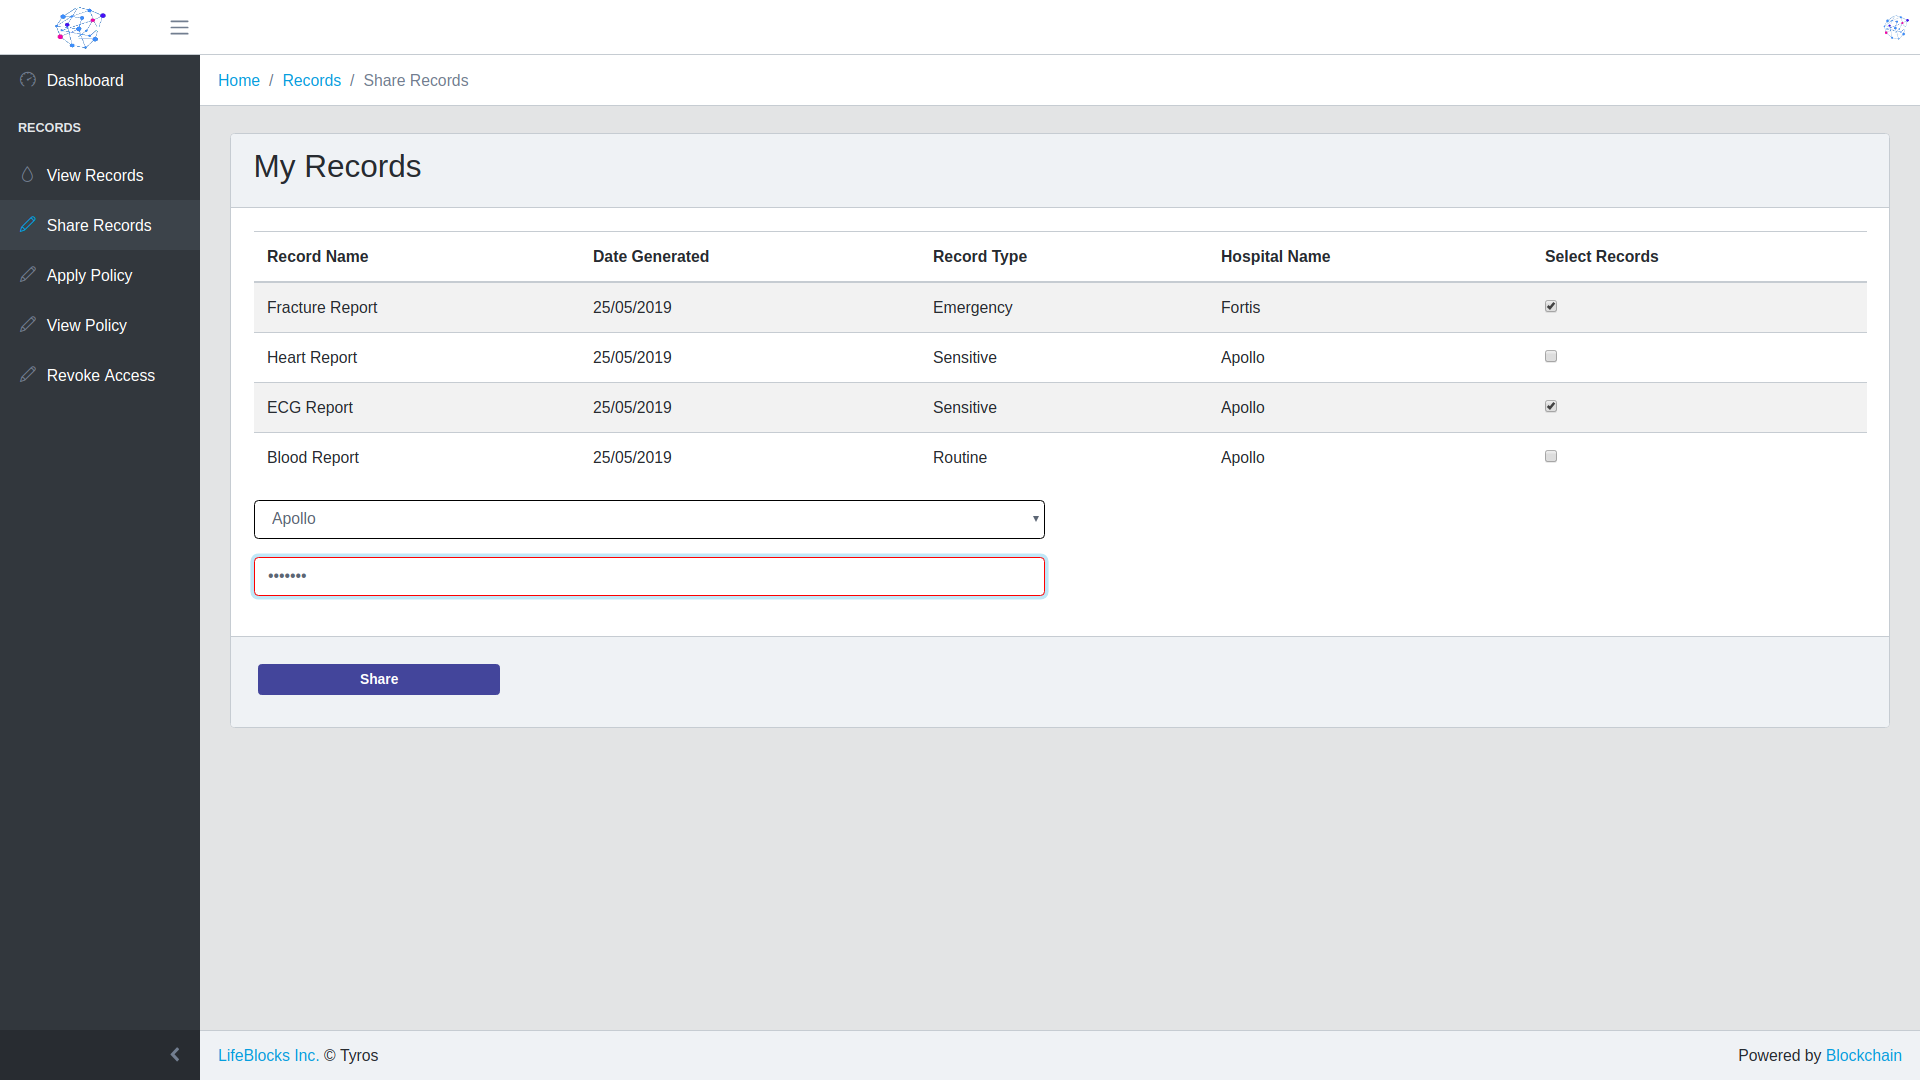
\includegraphics[width=\linewidth]{Images/User/UserShareRecord.png}
	\caption{ User Share Record}
	%\label{fig:universe}
\end{figure}


\begin{figure}[!b]
	\centering
	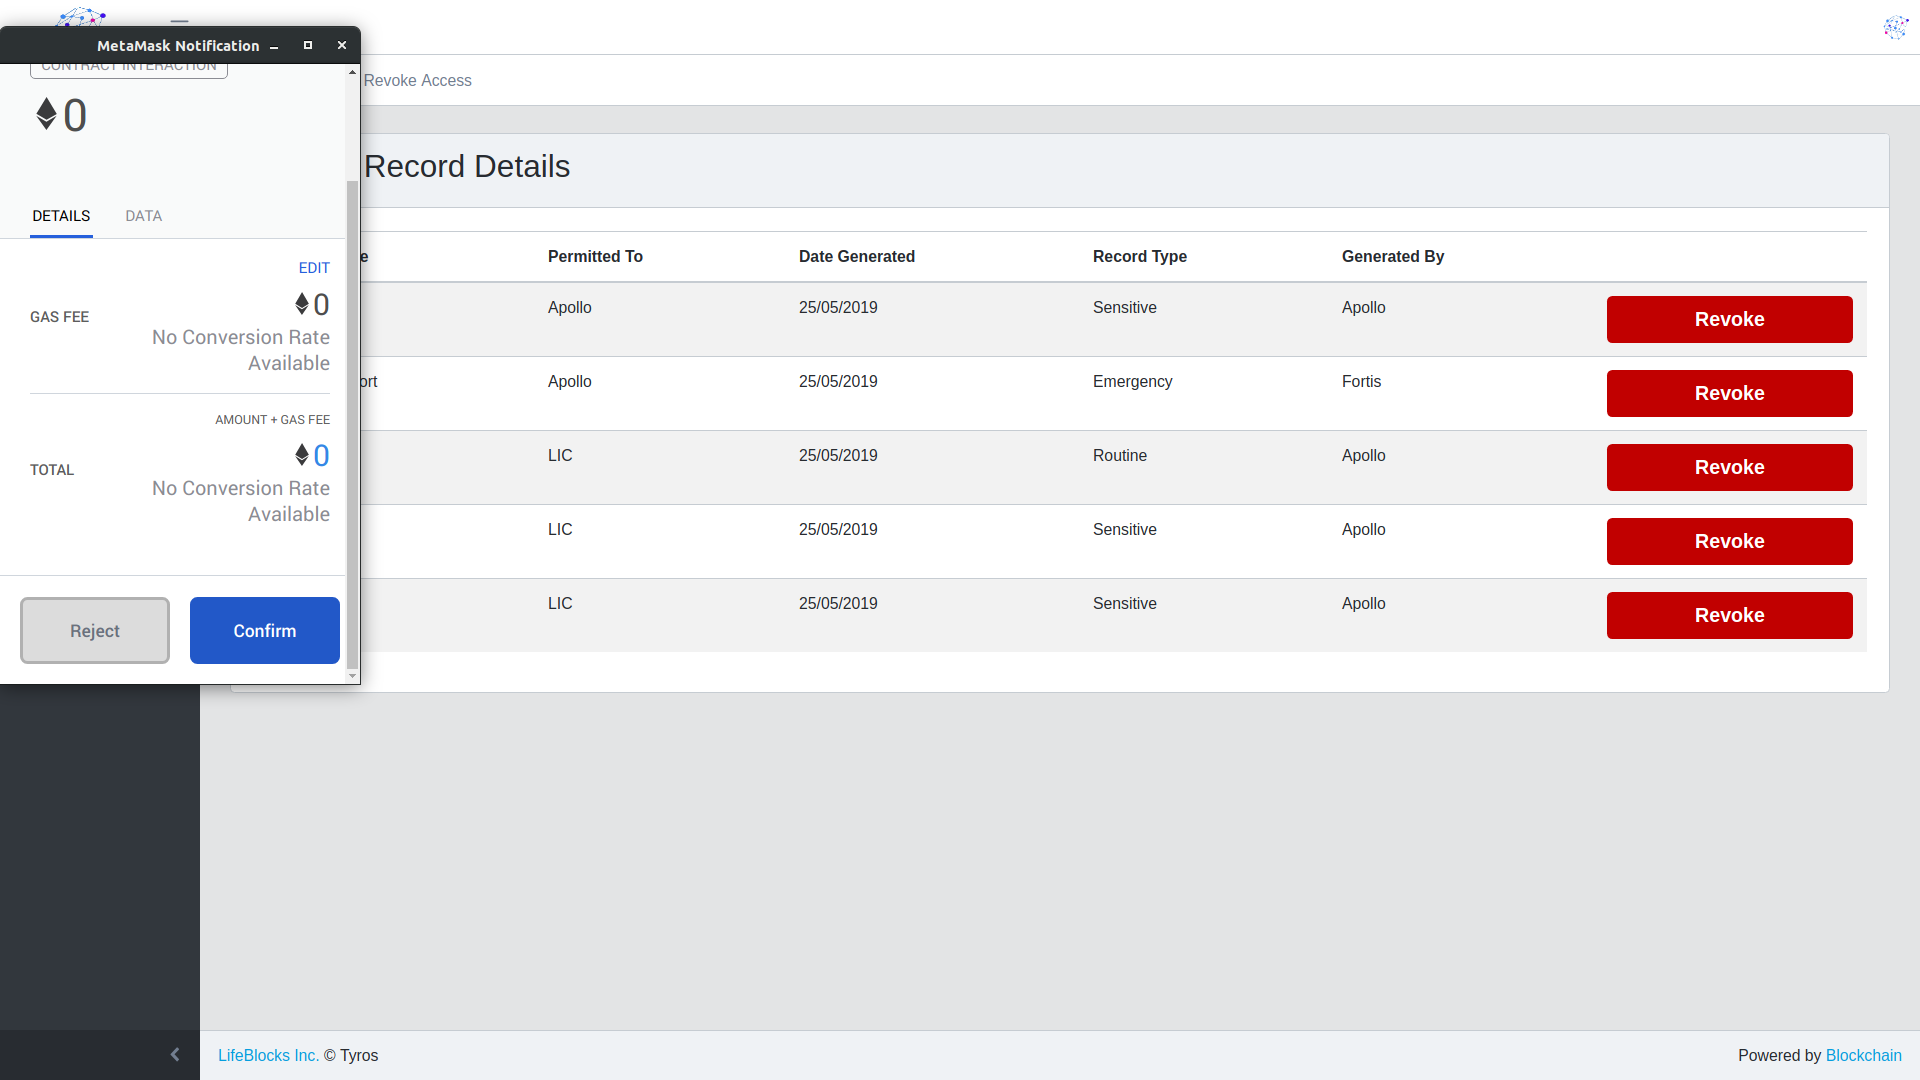
\includegraphics[width=\linewidth]{Images/User/UserRevokeRecordAccess.png}
	\caption{ User Revoke Record Access}
	%\label{fig:universe}
\end{figure}
\begin{figure}[!b]
	\centering
	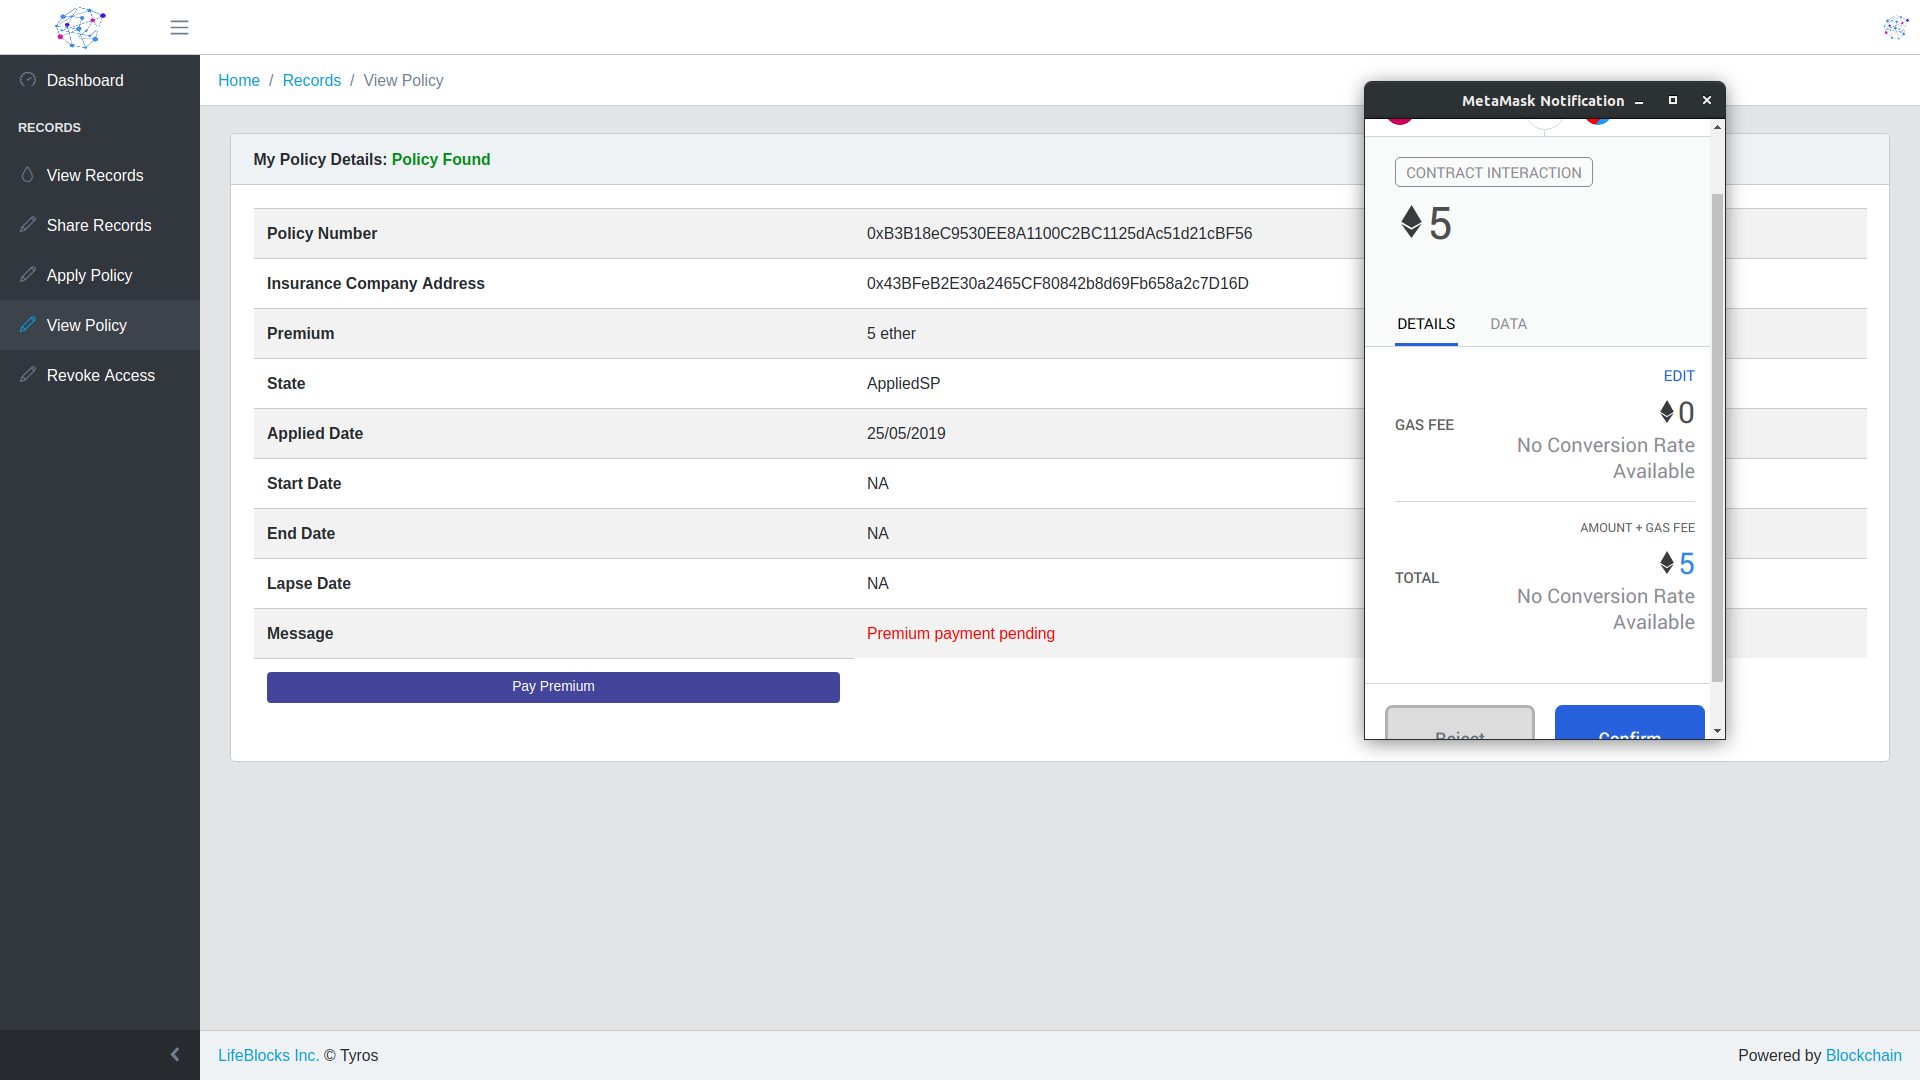
\includegraphics[width=\linewidth]{Images/User/UserPayPremium.png}
	\caption{ User Pay Premium}
	%\label{fig:universe}
\end{figure}

\begin{figure}[!b]
	\centering
	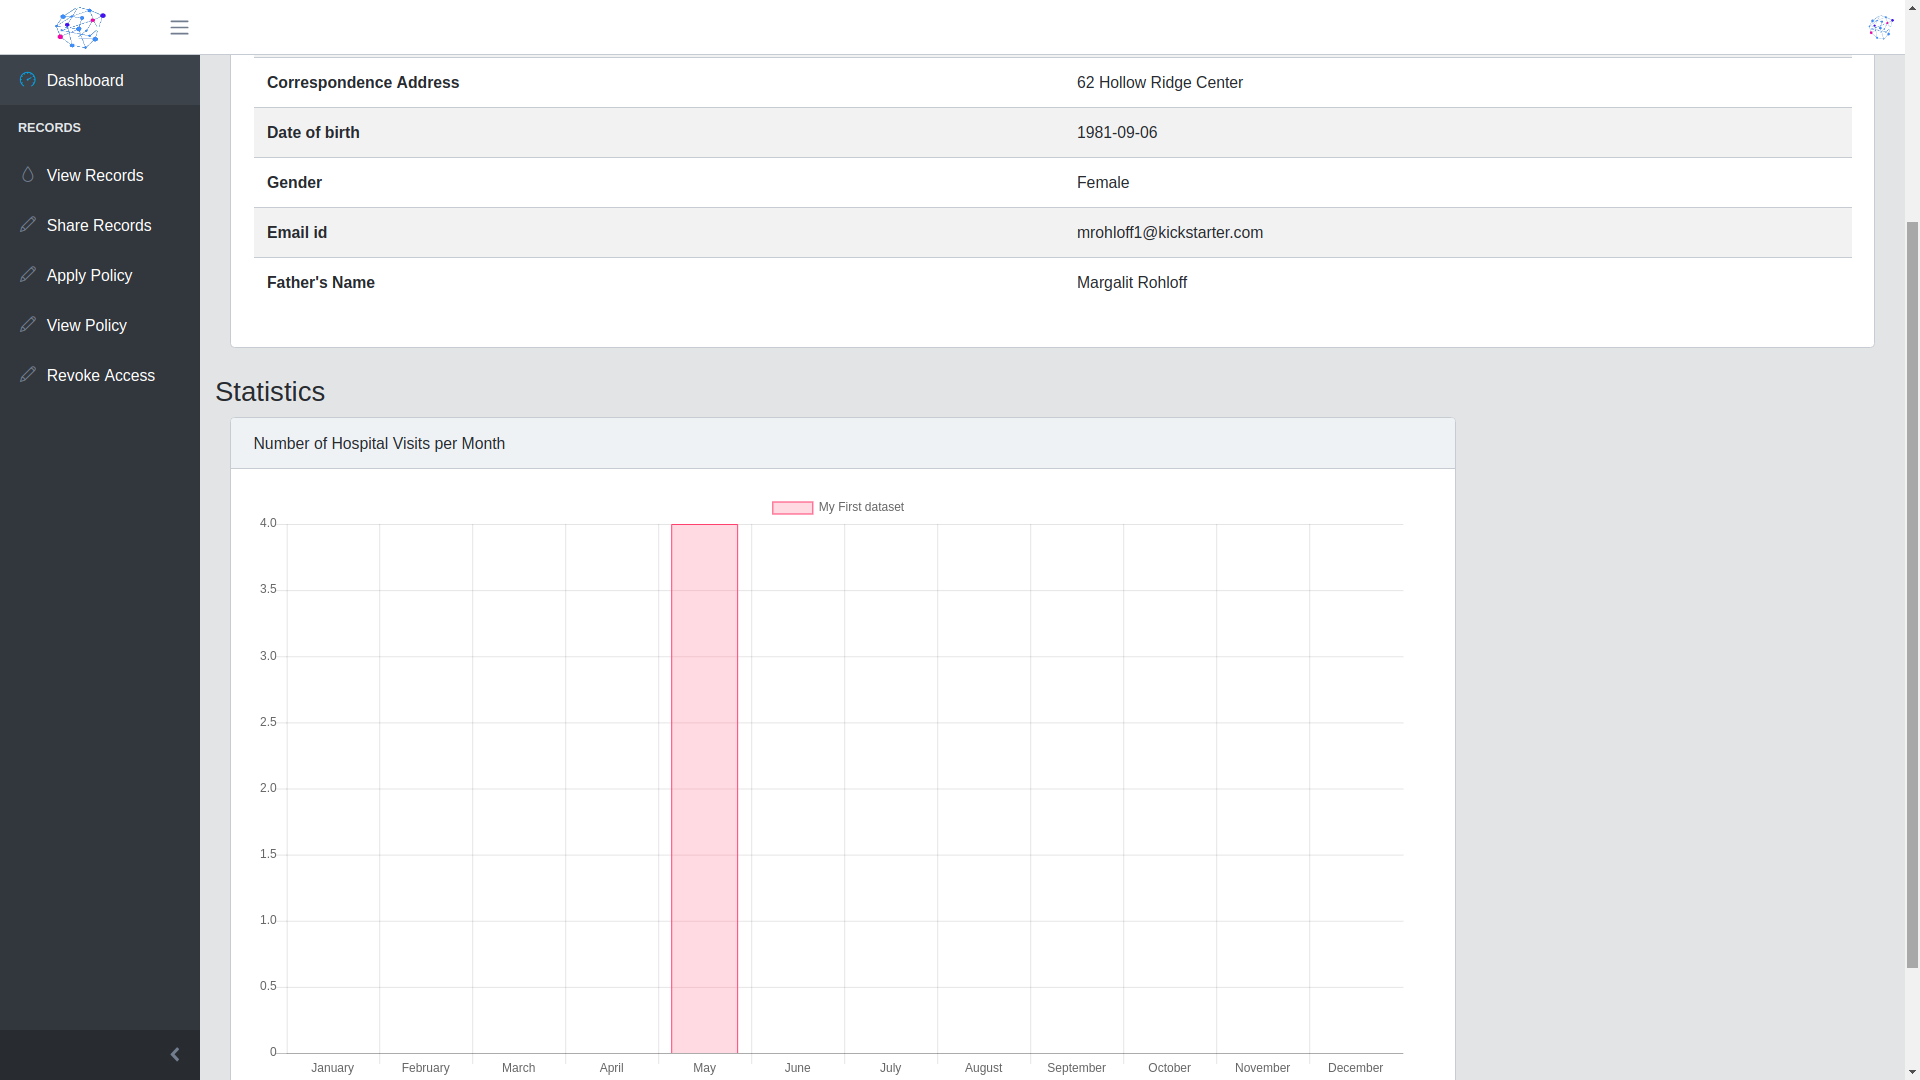
\includegraphics[width=\linewidth]{Images/User/UserStatistics.png}
	\caption{ User Statistics}
	%\label{fig:universe}
\end{figure}

\begin{figure}[!b]
	\centering
	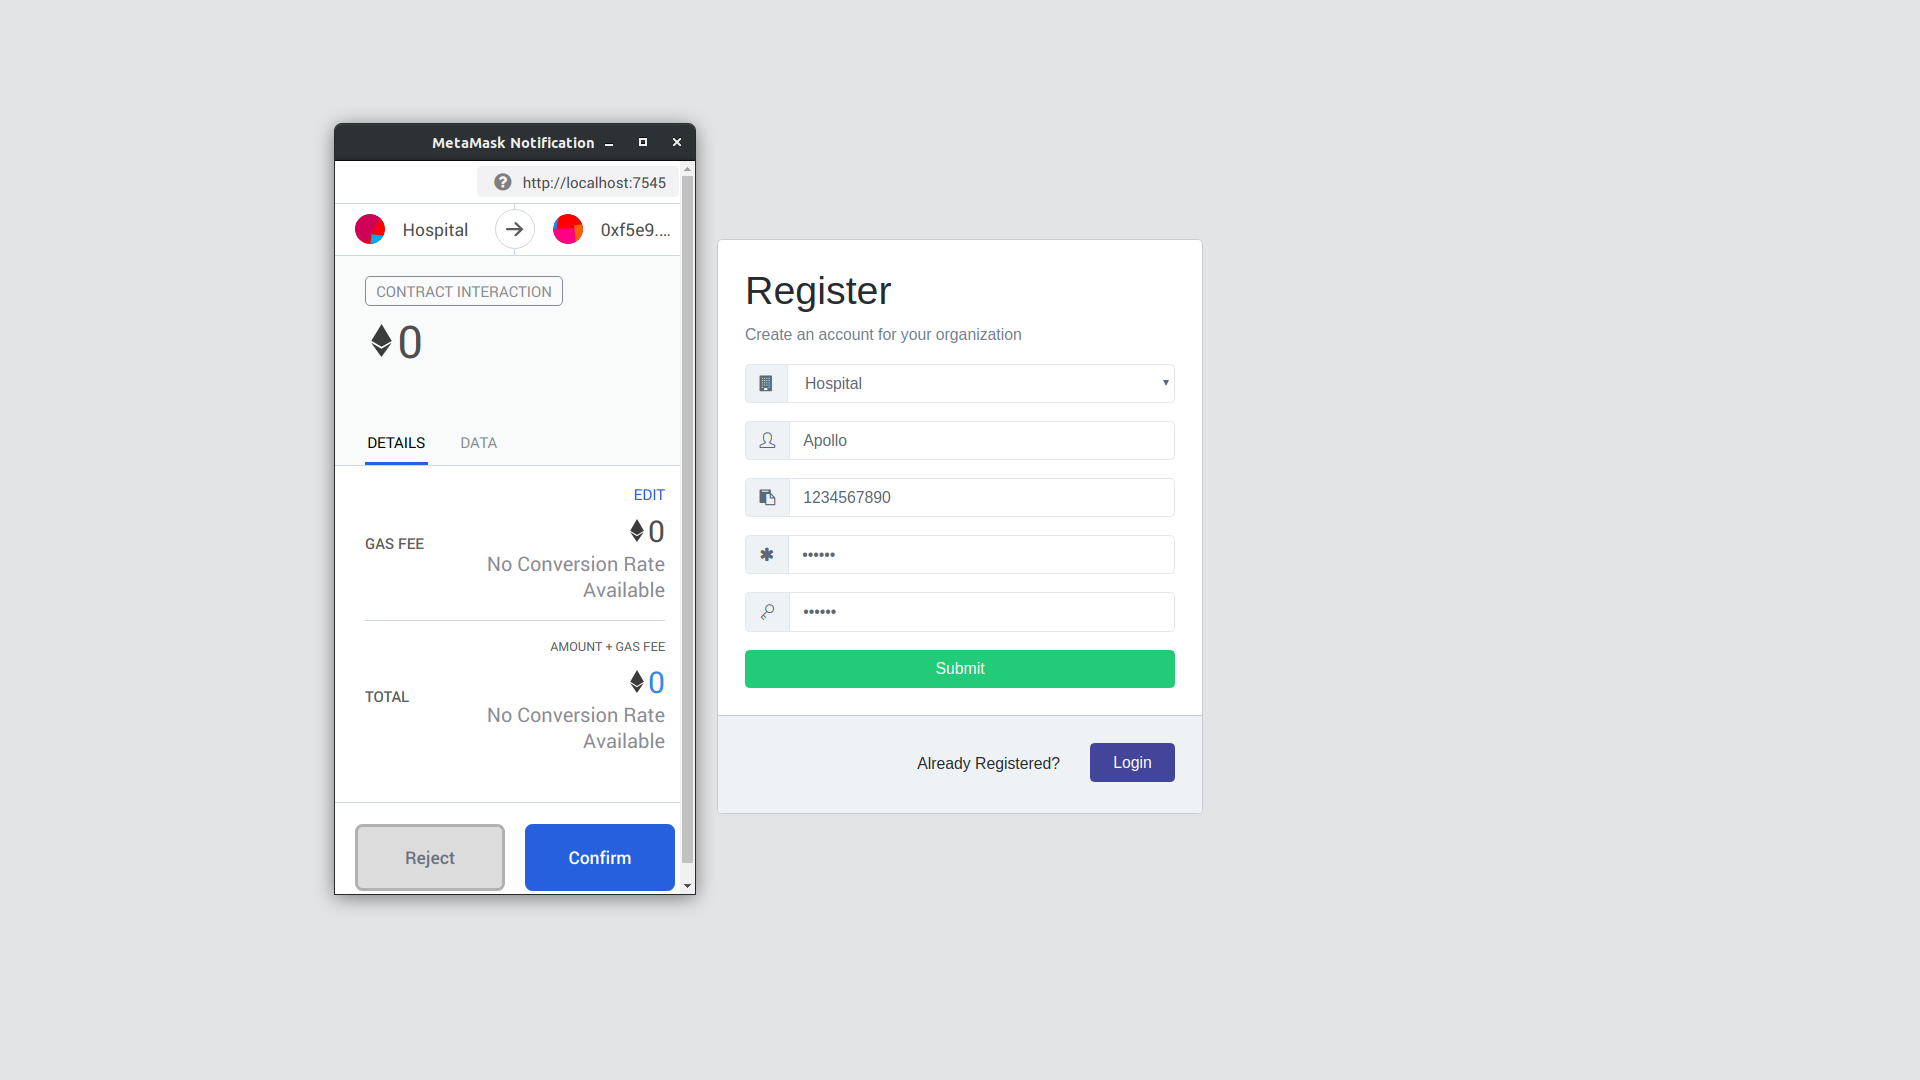
\includegraphics[width=\linewidth]{Images/Organisation/OrganizationRegister.png}
	\caption{ Organization Registration}
	%\label{fig:universe}
\end{figure}
\begin{figure}[!b]
	\centering
	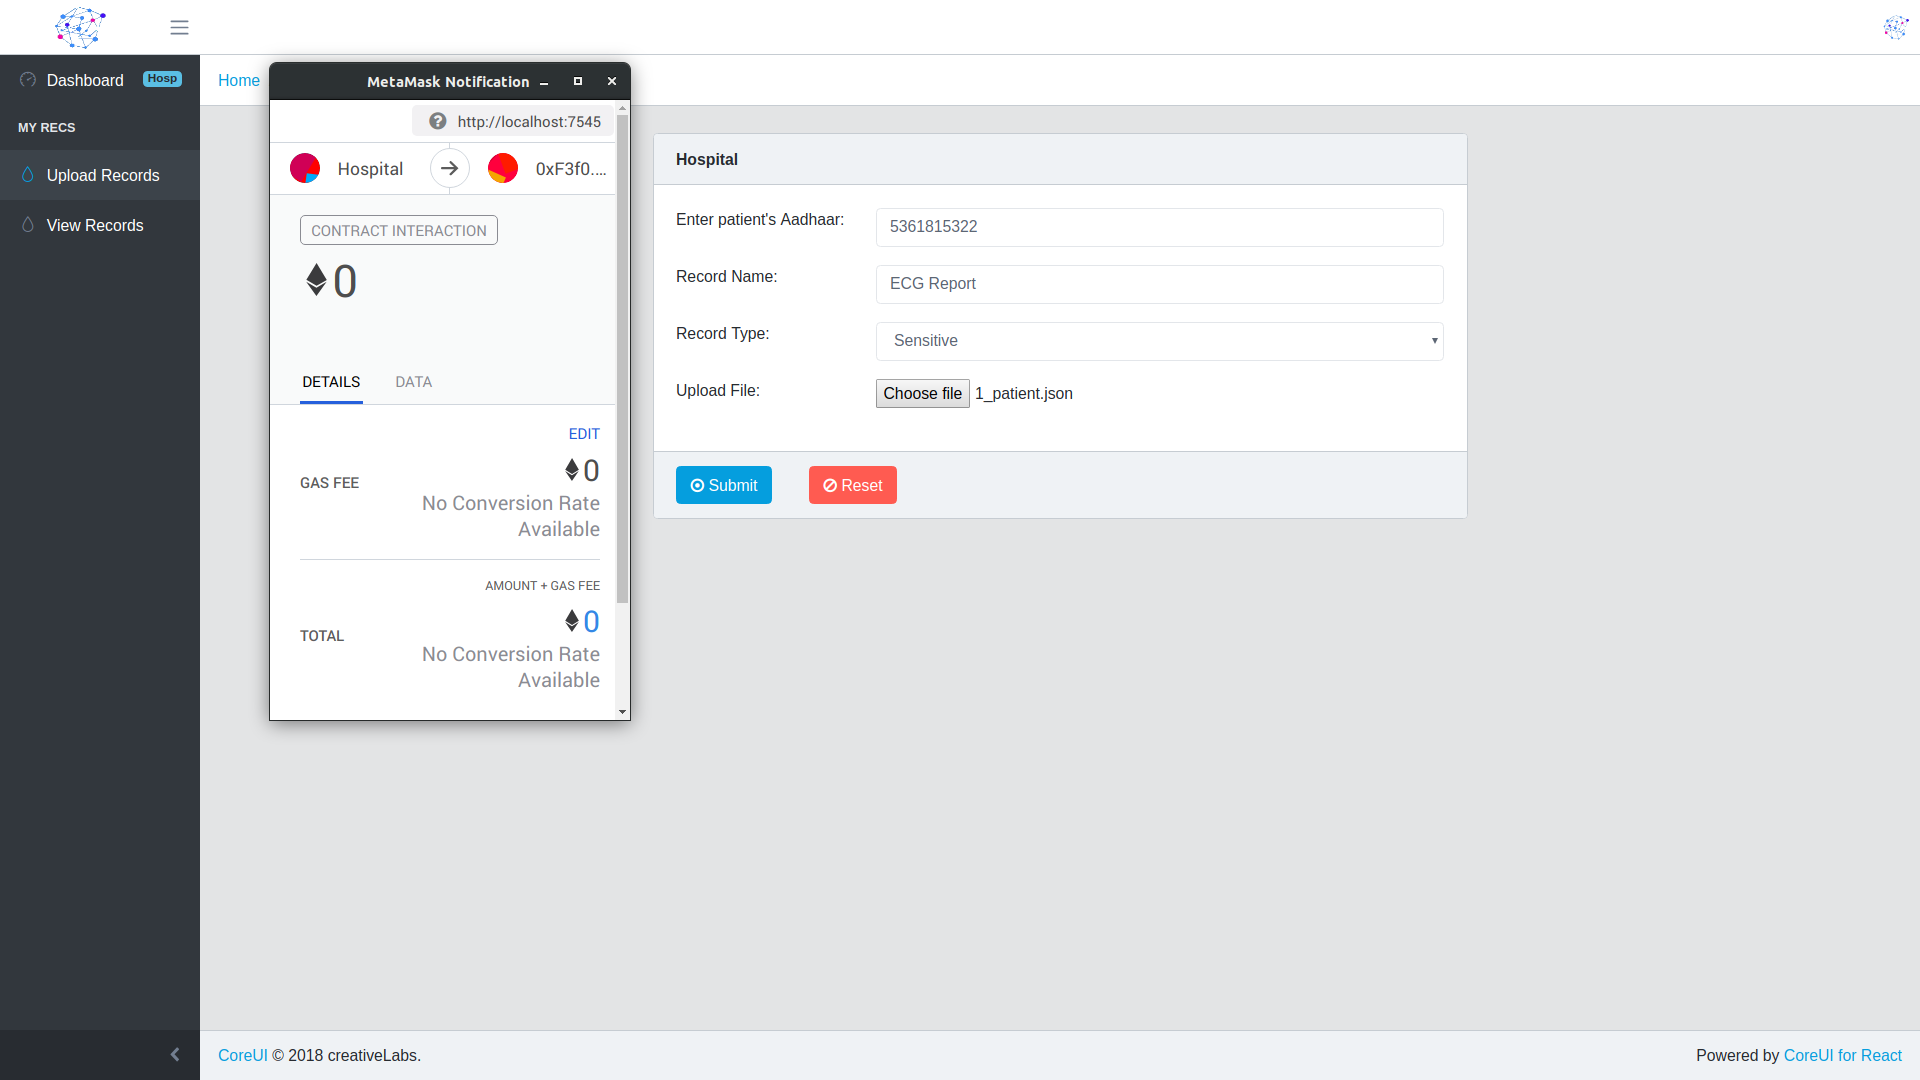
\includegraphics[width=\linewidth]{Images/Organisation/HospitalUploadRecord.png}
	\caption{ Hospital Upload Record}
	%\label{fig:universe}
\end{figure}


\begin{figure}[!b]
	\centering
	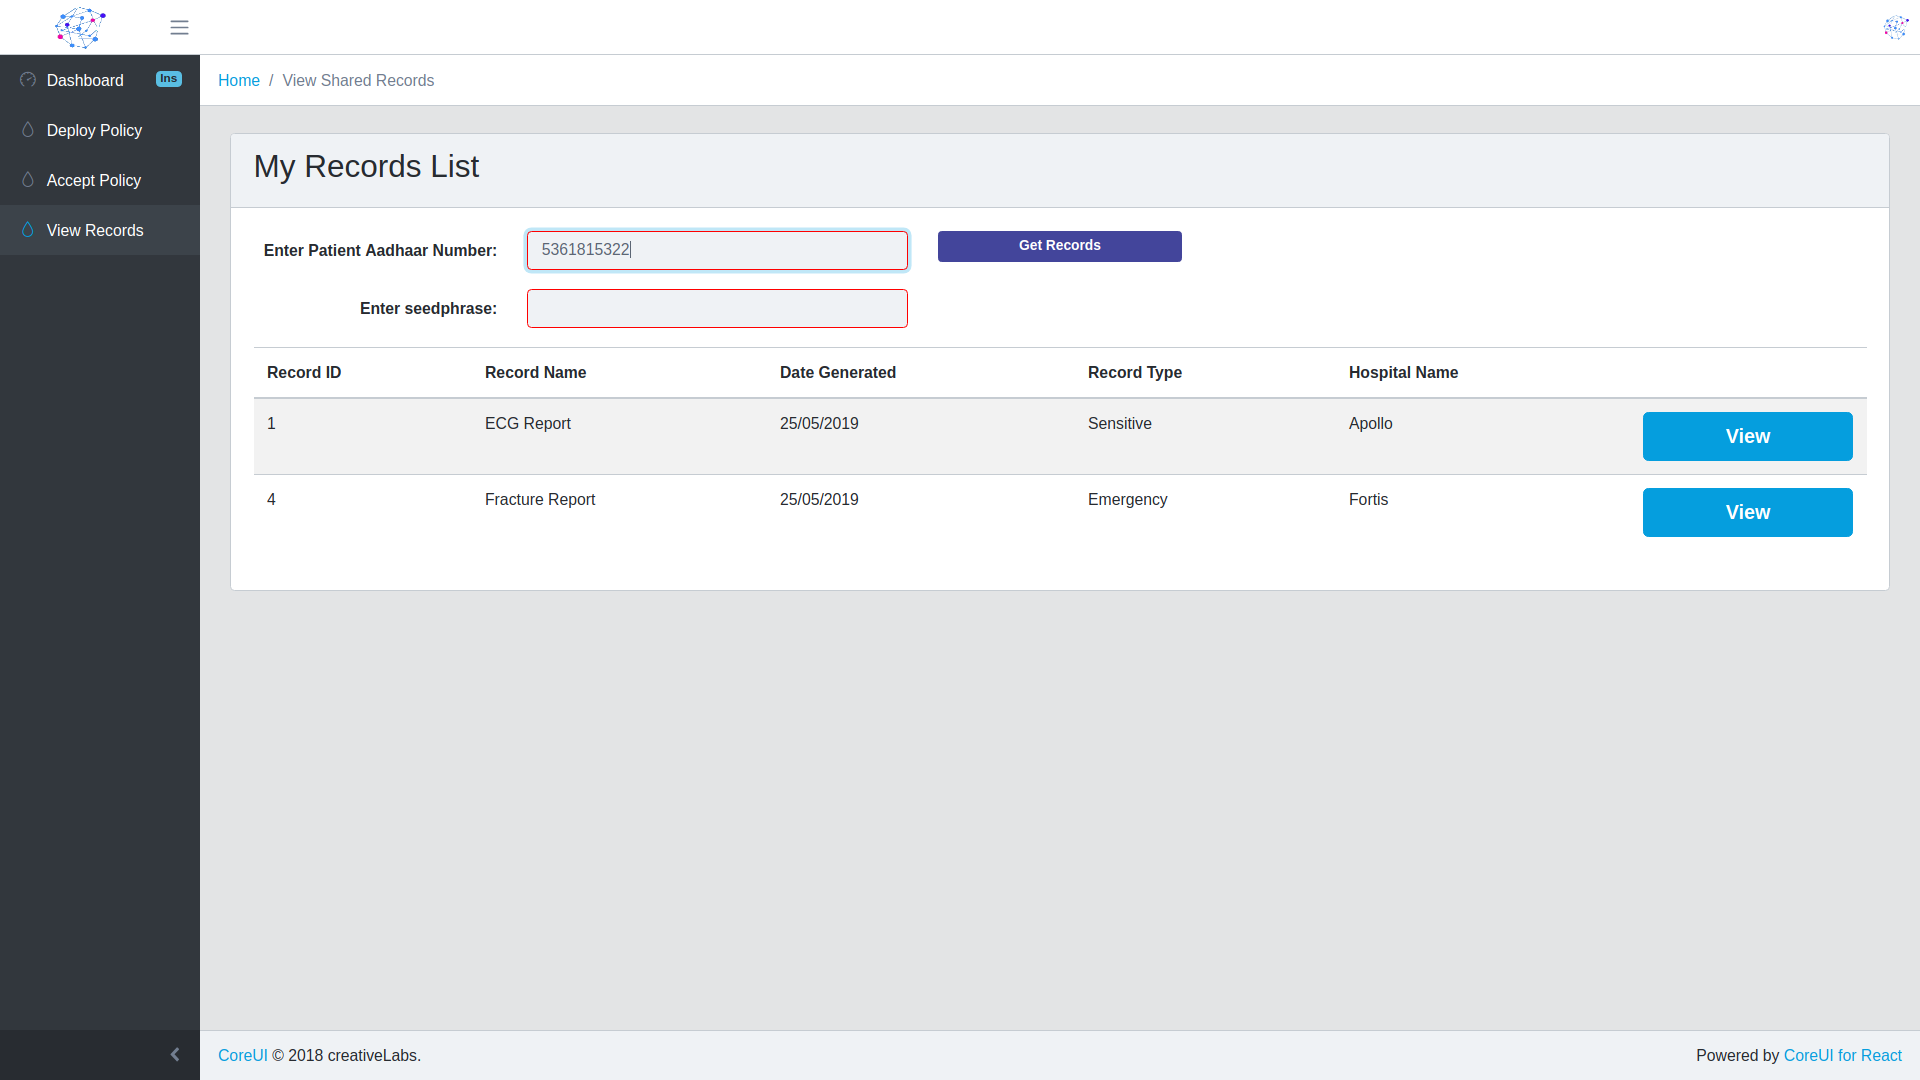
\includegraphics[width=\linewidth]{Images/Organisation/HospitalViewSharedRecords.png}
	\caption{ Hospital View Shared Records}
	%\label{fig:universe}
\end{figure}
\begin{figure}[!b]
	\centering
	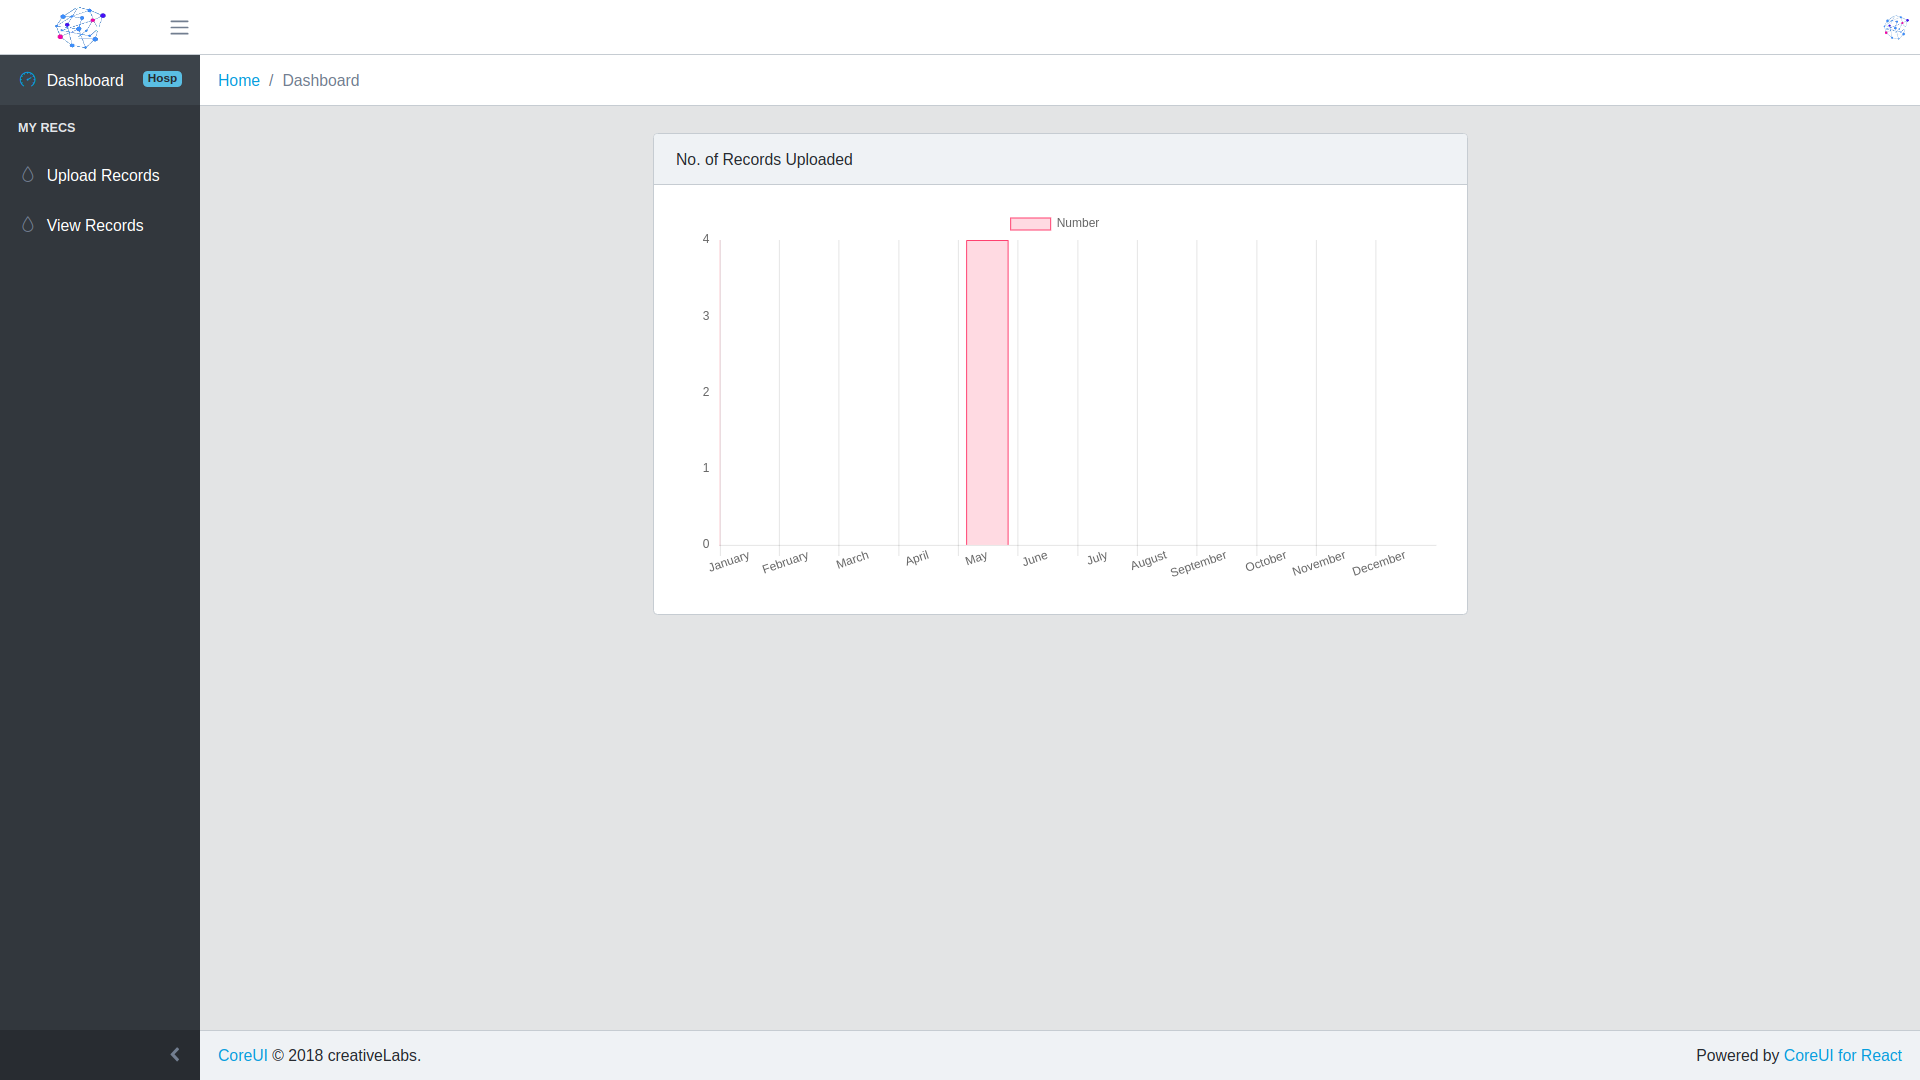
\includegraphics[width=\linewidth]{Images/Organisation/HospitalStatistics.png}
	\caption{ Hospital Statistics}
	%\label{fig:universe}
\end{figure}


\begin{figure}[!b]
	\centering
	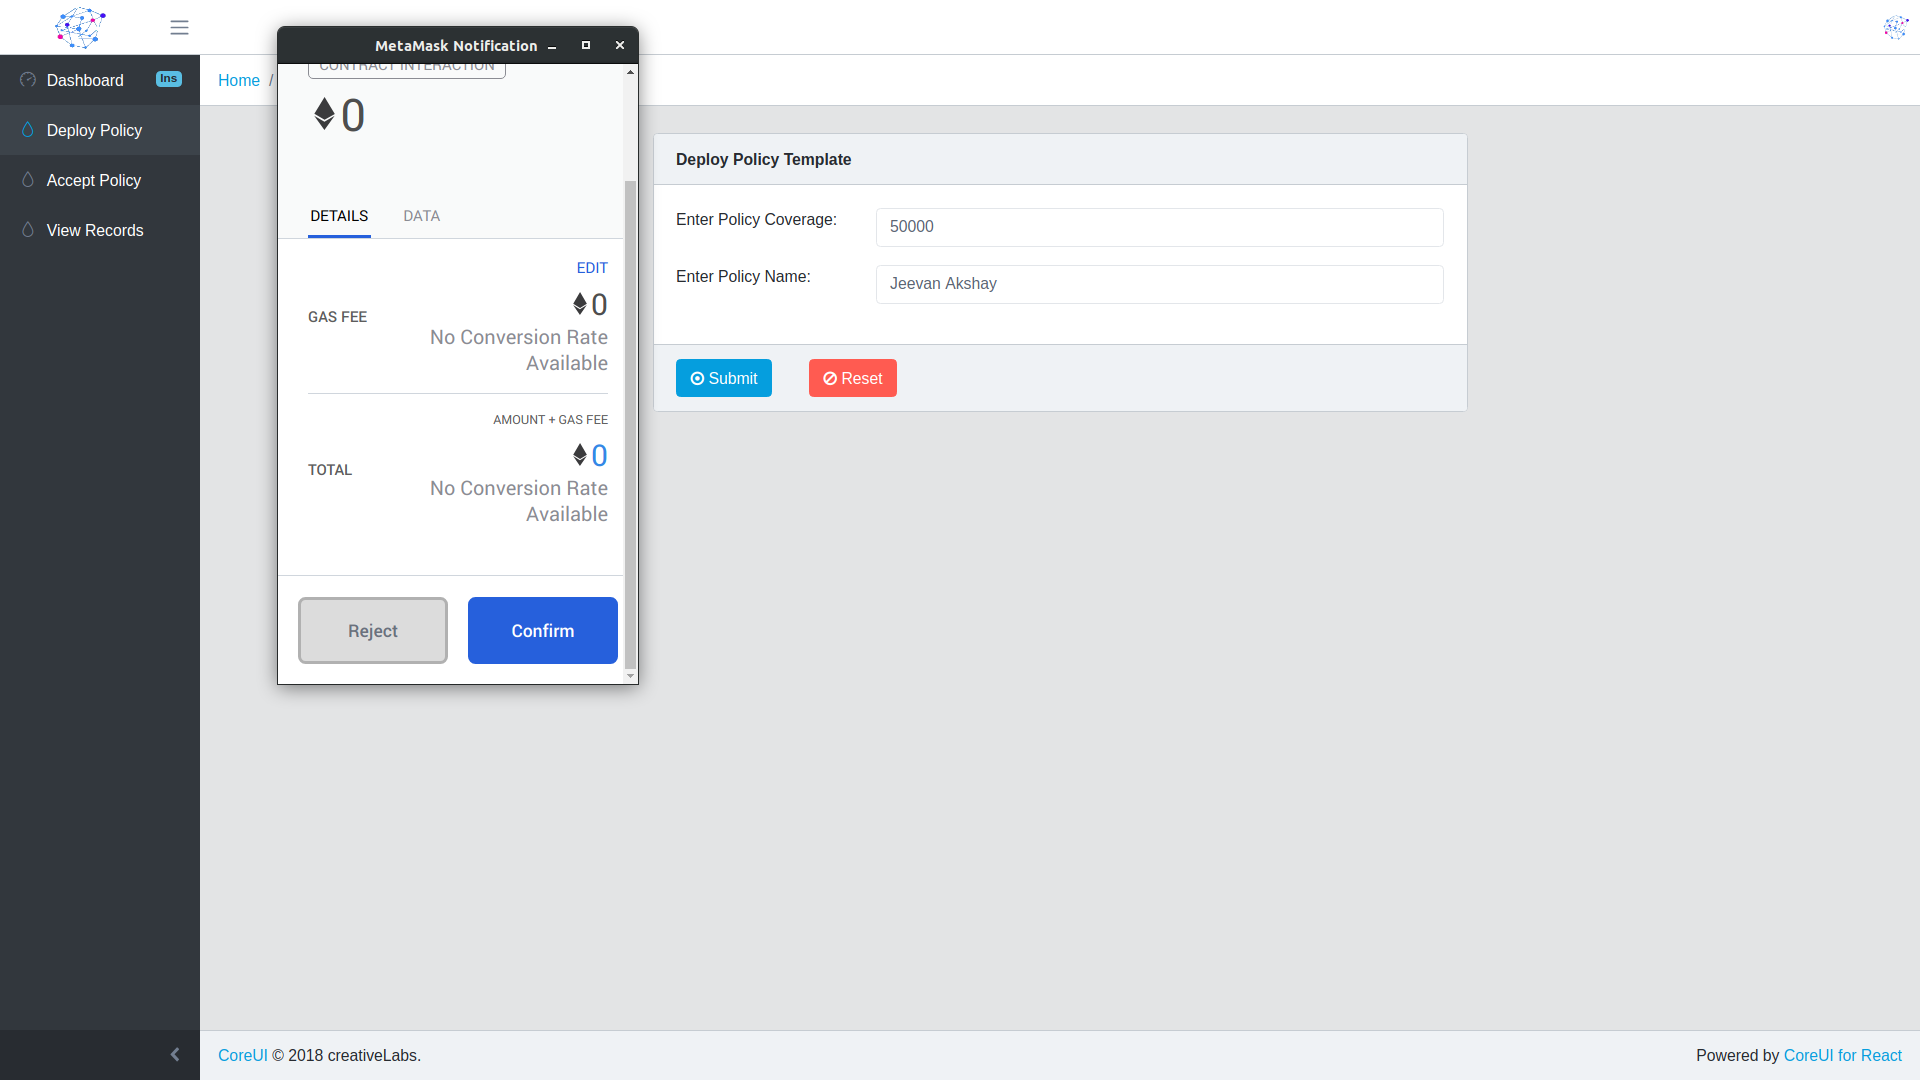
\includegraphics[width=\linewidth]{Images/Organisation/InsurancePolicyDeploy.png}
	\caption{Insurance Policy Deploy}
	%\label{fig:universe}
\end{figure}
\begin{figure}[!b]
	\centering
	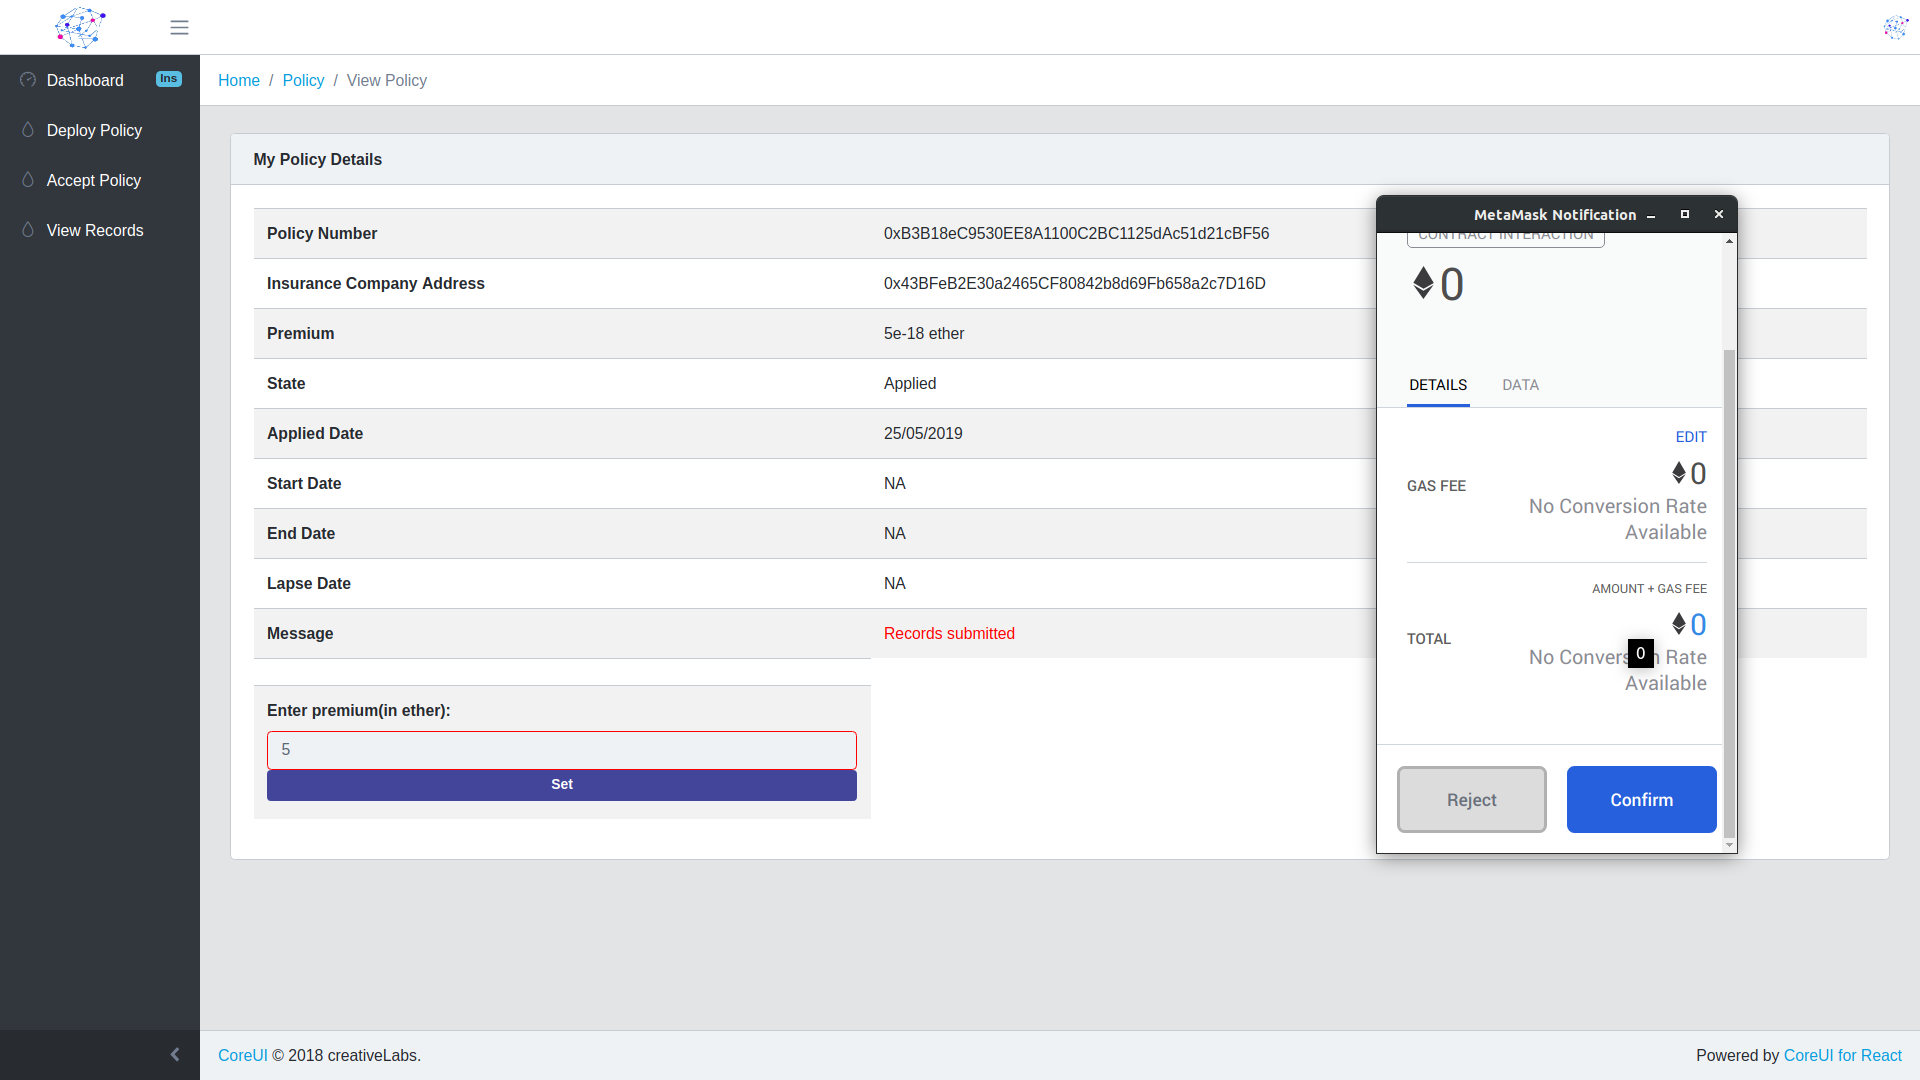
\includegraphics[width=\linewidth]{Images/Organisation/InsuranceAcceptPolicy.png}
	\caption{ User Share Record}
	%\label{fig:universe}
\end{figure}

\begin{figure}[!b]
	\centering
	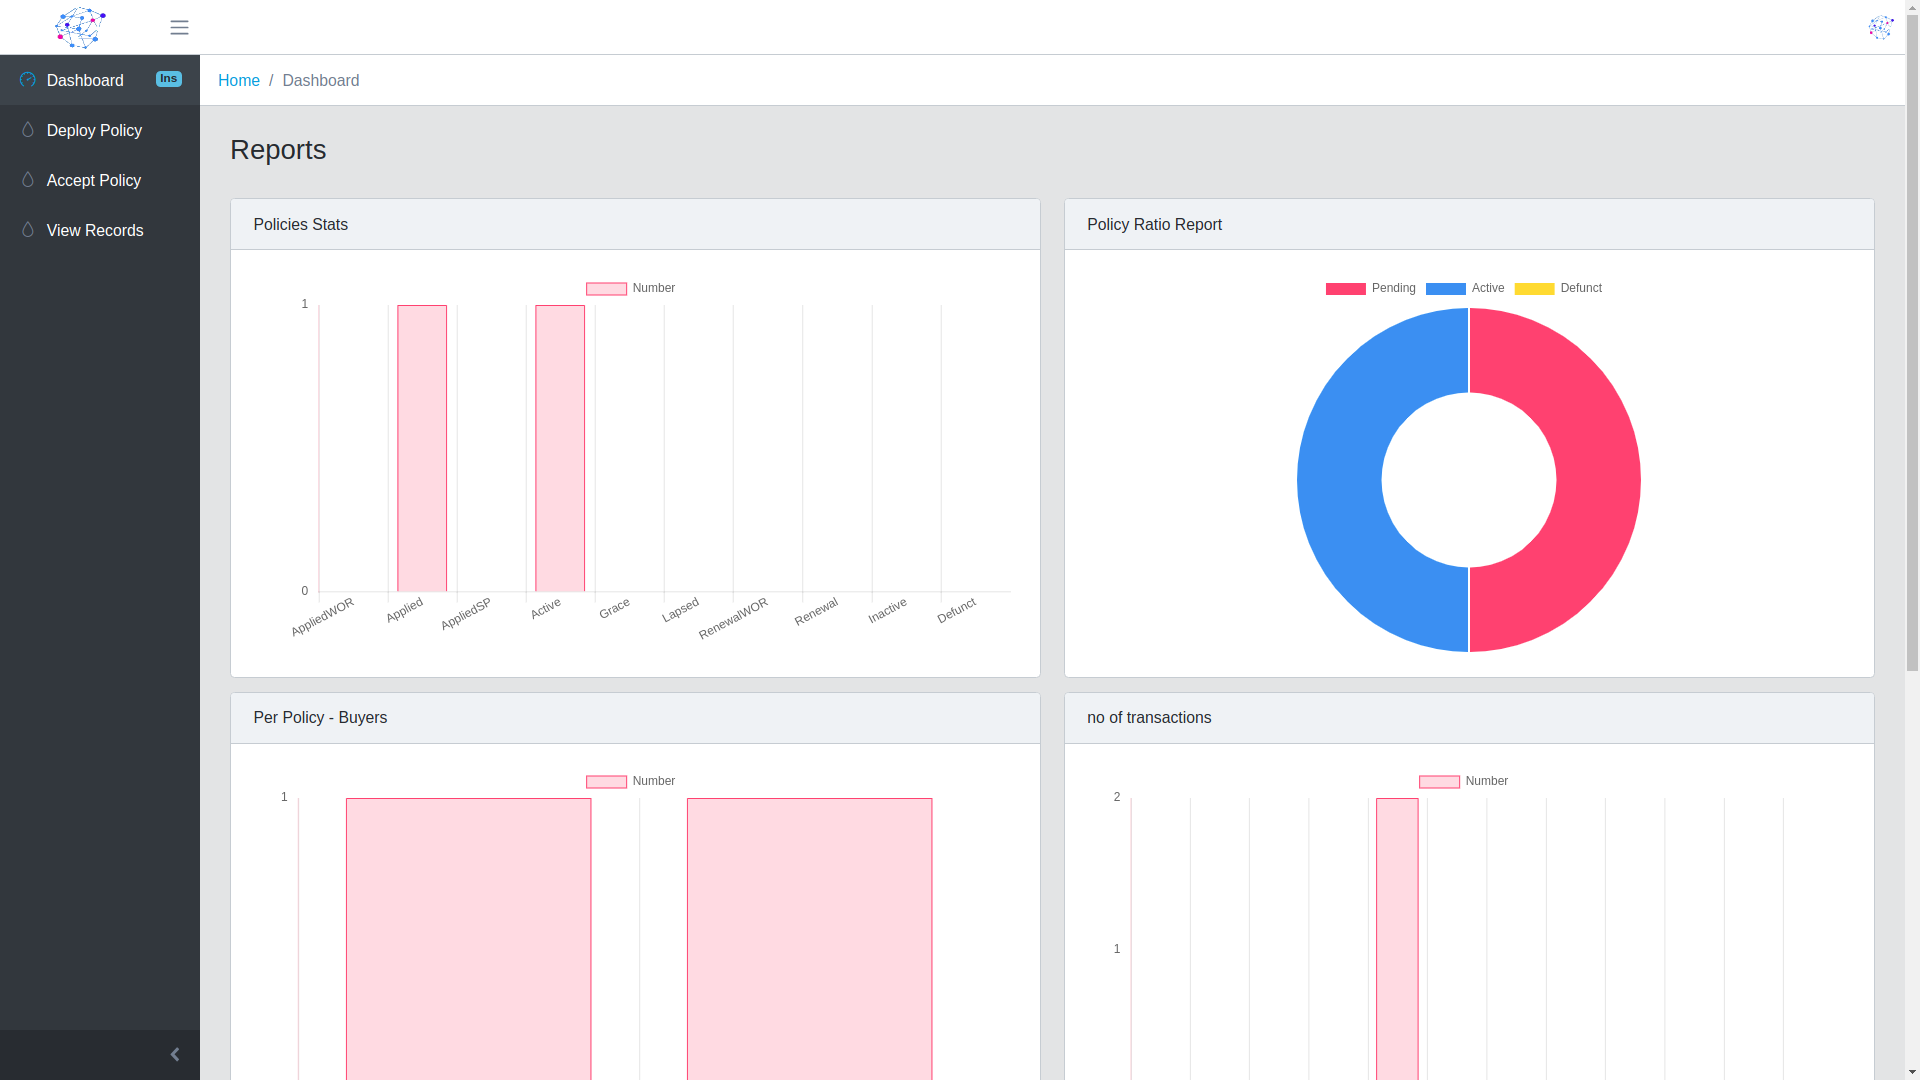
\includegraphics[width=\linewidth]{Images/Organisation/InsuranceCompanyStatistics1.png}
	\caption{Insurance Company Statistics }
	%\label{fig:universe}
\end{figure}
\begin{figure}[!b]
	\centering
	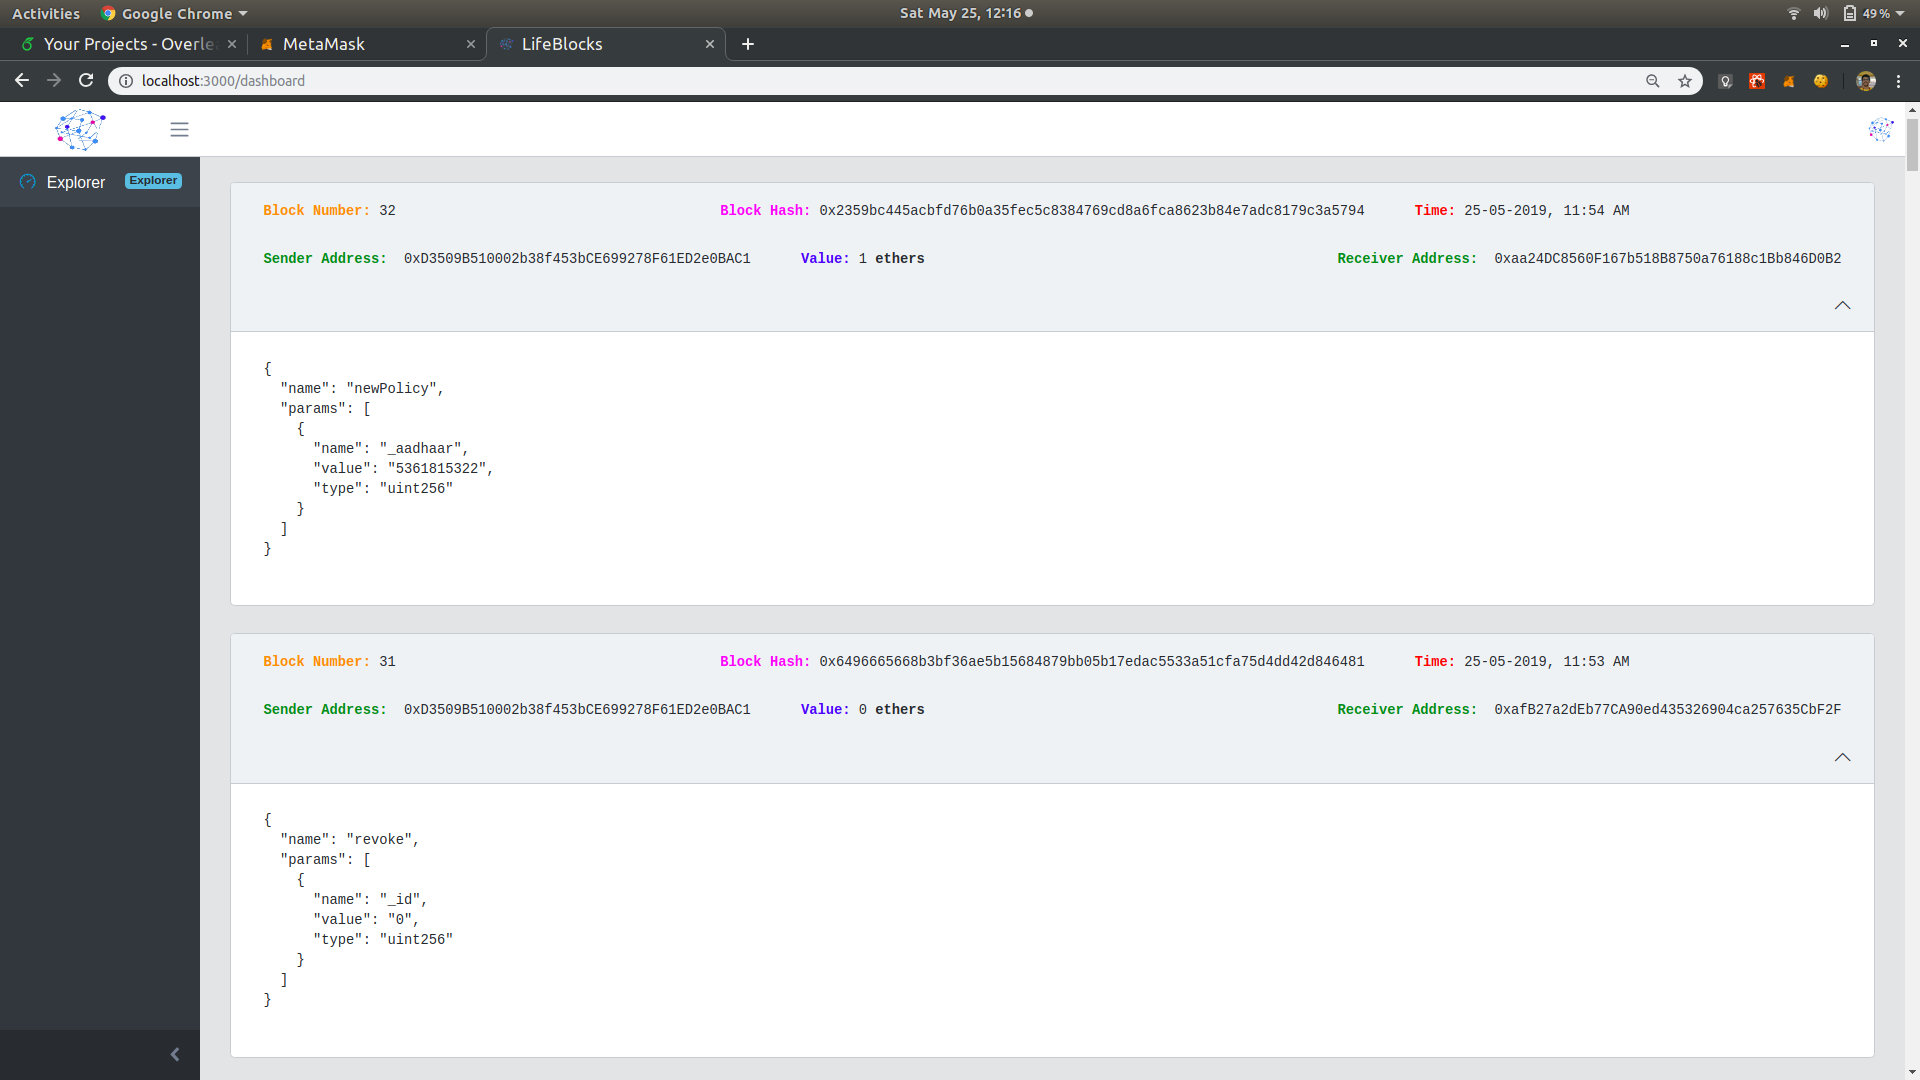
\includegraphics[width=\linewidth]{Images/Explorer/Screenshot1.png}
	\caption{Blockchain Explorer(a)}
	%\label{fig:universe}
\end{figure}
\begin{figure}[!b]
	\centering
	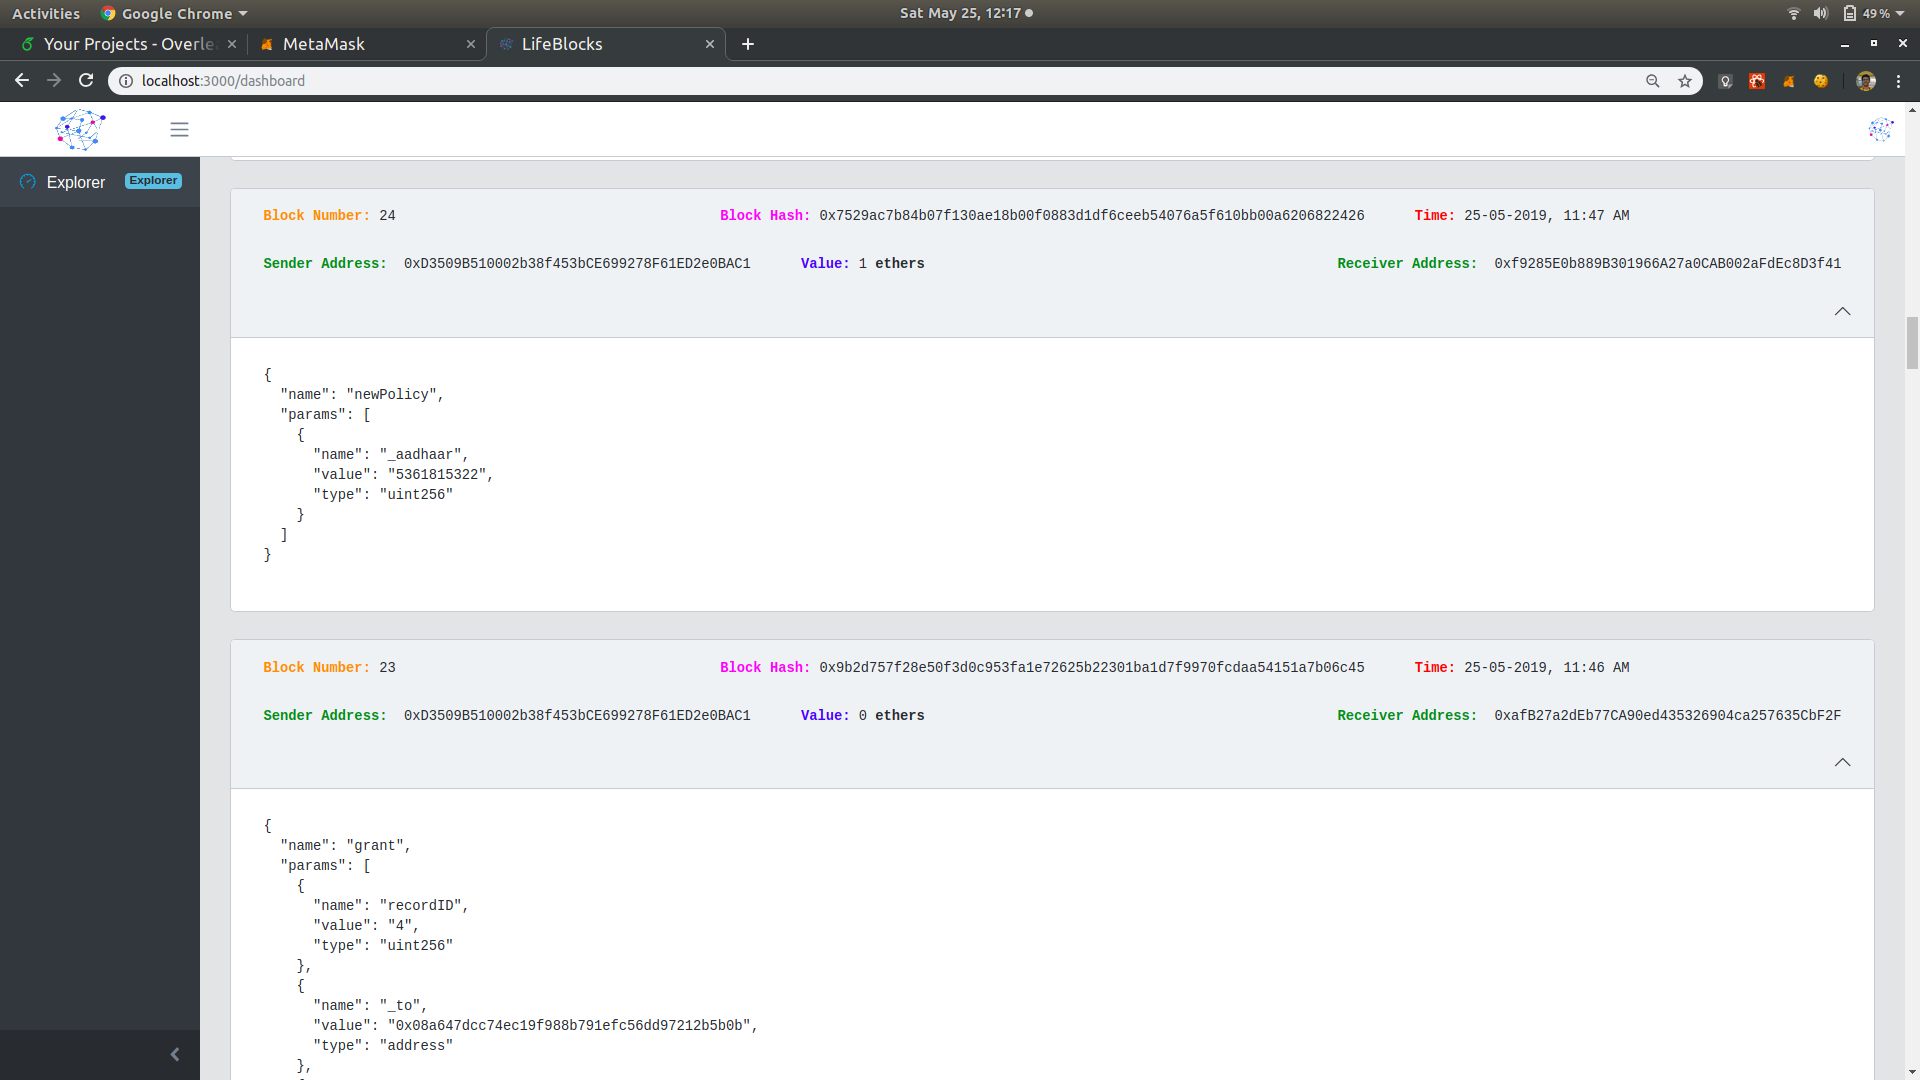
\includegraphics[width=\linewidth]{Images/Explorer/Screenshot2.png}
	\caption{Blockchain Explorer(b) }
	%\label{fig:universe}
\end{figure}

\clearpage
\section{Code Snippets}
\lstset{caption={Chai_spec.json}}
\begin{lstlisting}[frame=single]  
$${
"name": "LifeBlocks",
"engine": {
    "authorityRound": {
        "params": {
            "stepDuration": "5",
            "validators" : {
                "list": [
                "0x0062b5a1d7b9f607e01057c71968908f1a3dc880",
                "0x00fbe91ac230841243cfb0a9c4fa2201310736f1",
                "0x00a06e9d56e1459fe0dfdf4c7db382425cc09448",
                "0x00edb55942d75eef1d88fabf6e0190b582386a80"
                    ]
                }
            }
        }
    },
    "params": {
        "gasLimitBoundDivisor": "0x400",
        "maximumExtraDataSize": "0x20",
        "minGasLimit": "0x1388",
        "networkID" : "0x2323",
        "eip155Transition": 0,
        "validateChainIdTransition": 0,
        "eip140Transition": 0,
        "eip211Transition": 0,
        "eip214Transition": 0,
        "eip658Transition": 0
      },
      }$$
      \end{lstlisting}
      \clearpage
\begin{lstlisting}[frame=single]  
    "genesis": {
        "seal": {
            "authorityRound": {
             "step": "0x0",
             "signature": "0x000000000000000000000000000000000
              0000000000000000000000000000000000000000000000000
              000000000000000000000000000000000000000000000000"
            }
        },
        "difficulty": "0x20000",
        "gasLimit": "0x5B8D80"
    },
    "accounts": {
    "0x0000000000000000000000000000000000000001":
    { "balance": "1", "builtin": { "name": "ecrecover",
    "pricing": { "linear": { "base": 3000, "word": 0 } } } },
    "0x0000000000000000000000000000000000000002":
    { "balance": "1", "builtin": { "name": "sha256", 
    "pricing": { "linear": { "base": 60, "word": 12 } } } },
    "0x0000000000000000000000000000000000000003":
    { "balance": "1", "builtin": { "name": "ripemd160",
    "pricing": { "linear": { "base": 600, "word": 120 } } } },
    "0x0000000000000000000000000000000000000004": 
    { "balance": "1", "builtin": { "name": "identity", 
    "pricing": { "linear": { "base": 15, "word": 3 } } } }
    }\end{math}
\end{lstlisting}
\clearpage
\lstset{caption={Config.toml file}}
\begin{lstlisting}[frame=single]  

[parity]
chain = "genesis.json"
base_path = "/home/parity/LifeBlocks"
[network]
port = 30300
[rpc]
port = 7545
apis = ["web3", "eth", "net", "personal", "parity", "parity_set"
,"traces", "rpc", "parity_accounts"]
cors = ["all"]
[websockets]
port = 7455
[account]
password = ["account.pwds"]
[mining]
engine_signer = "0x0062b5a1d7b9f607e01057c71968908f1a3dc880"
reseal_on_txs = "none"

\end{lstlisting}
\clearpage
\lstset{caption={UserDetails Smart Contract}}
\begin{lstlisting}[frame=single]

pragma solidity ^0.4.24;

contract userDetails{
  
   event addressLinked(address _address, uint _aadhaar);
   event keyLinked(address _address, string _ipfshash);

   mapping(uint => address) public aadhaarToAddress;
   mapping(address => uint) public addressToAadhaar;
   mapping(address => string) public ownerToKey;
   mapping(uint => address) public ownerToPolicy;
    
   function link(uint _aadhaar, string _ipfskey) public{
       require(aadhaarToAddress[_aadhaar] ==
       0x0000000000000000000000000000000000000000,
       "Aadhar Card already exists");
       require(addressToAadhaar[msg.sender] == 
       0,"Address already used");
       require(bytes(ownerToKey[msg.sender]).length == 0,
       "Key pair for user already exists");
       aadhaarToAddress[_aadhaar] = msg.sender;
       addressToAadhaar[msg.sender] = _aadhaar;
       emit addressLinked(msg.sender, _aadhaar);
       ownerToKey[msg.sender] = _ipfskey;
       emit keyLinked(msg.sender, _ipfskey);      
   }
.
.
.
.
 }

\end{lstlisting}

\clearpage
\lstset{caption={ReactJS}}
\begin{lstlisting}[frame=single]
import React, { Component } from 'react'
import ipfs from '../../../Dependencies/ipfs'
import {decrypt} from '../../../Dependencies/crypto'

export class ViewPolicy extends Component {
    constructor(props) {
      super(props)
      this.state = {
        userAddress : '',
        selectValue: '',
        account: null,
        };
 }

      async componentWillMount() {        
        await this.instantiateContract()
      }

     async instantiateContract() {
        //User Details Contract Instantiation
      const contractAddress_u = userdetails.contract_address       
      const ABI_u = userdetails.abi              
      var UserContract = new this.state.web3.eth.Contract(ABI_u,
      contractAddress_u)     
      this.UserContract = UserContract
      
      //Organization Contract Instantitation
      const orgContractAddress = organization.contract_address
      const orgABI = organization.abi
      var orgContract = new this.state.web3.eth.Contract(orgABI,
      orgContractAddress)
      this.orgContract = orgContract
      \end{lstlisting}
    \clearpage
    \begin{lstlisting}[frame=single]  
      //Get account from metamask
          await this.state.web3.eth.getAccounts
          ((error,accounts)=> {
          if(!error) {
            console.log(accounts[0])
            this.setState({
              account: accounts[0]
            })
            this.viewPolicy()
          }
          else {
            console.log(error)
          }
   
        })              
      }
  
     viewPolicy() {
      document.getElementById("policy").style.display = "none"
      this.state.web3.eth.getAccounts((error, accounts) => {
        //get the account from metamask 
        this.UserContract.methods.login(sessionStorage.getItem
        ('aadhaar')).call(
          { from: accounts[0] },
          (error, x)=> {
            //check if account exists
            if (error) {
              alert("Wrong");
              return;
            }
               \end{lstlisting}
    \clearpage
    \begin{lstlisting}[frame=single]  
            if (x === true) {
              //get address from aadhaar number
              this.UserContract.methods
                .getAddress(sessionStorage.getItem('aadhaar'))
                .call(
                  { from: accounts[0] },
                  (error, add) => {
                    //get account address from SC
                    if (error) {
                      alert("Wrong Details");
                      return;
                    }    
            ....    
     }
   render() {   
    return (
      <div className="animated fadeIn">         
           <Row>
          <Col md="9" lg="12" xl="12">
        <Card>    
          <CardHeader>
           ...
        <tr>
          <td><strong>Policy Number</strong></td>
          <td>{this.state.policyAddress}</td>
        </tr>
        <tr>
          <td><strong>Insurance Company Address</strong></td>
          <td>{this.state.policyDetails[0]}</td>
        </tr>
        <tr>
          <td><strong>Premium</strong></td>
          <td>{this.state.premium}</td>
             \end{lstlisting}
\section{Experimental Setup}
All the experiments are executed on a laptop equipped with 8GB DDR3 RAM ,Intel Dual Core i5-7200U CPU @ 2.50GHz running Linux in 64-bit mode.The system has Ganache installed on it, which is a local blockchain provider and can be used to run tests, execute commands, and inspect state while controlling how the chain operates. The distributed applications for a customer, hospitals, a insurance providers are run on different ports of the laptop and the frontend is designed using React.Transactions initiated on the frontend are relayed through MetaMask which is a bridge between blockchain provider and the distributed application.Transaction details of scheduled transactions are stored in MySQL and these transactions are scheduled as jobs on MongoDB via a listener and stored for persistence.
\clearpage \section{Test Cases}
Test Cases For a Customer\\
% \begin{table}[]
%     \centering
%     \begin{tabular}{|c|c|c|c|c|} 
% \hline
%  \textbf{Test ID} & \textbf{Test Description} &\textbf{Input} & \textbf{Expected Result} & \textbf{Actual Output} \\ \hline \scriptsize 1 &\scriptsize Register with Ethereum Address& cell6 & \\ \hline 
%  2 & cell8 & cell9 &&\\ \hline \scriptsize
%  2 & cell8 & cell9 &\\ \hline \scriptsize
%  2 & cell8 & cell9 &\\ \hline \scriptsize
%  2 & cell8 & cell9 &\\ \hline \scriptsize
%  2 & cell8 & cell9 &\\ \hline
% \end{tabular}
%     \caption{Caption}
%     %\label{tab:my_label}
% \end{table}

\begin{table}[h!]
	\begin{tabular}{|p{.65cm}|p{2.5cm}|p{3.5cm}|p{3cm}|p{3.5cm}|}
		\hline
		\centering\textbf{Test ID} & \centering\textbf{Test Description} & \centering\textbf{Input} & \centering\textbf{Expected Result} & \textbf{Actual Output} \\ \hline
 
		\multirow{2}{1em}{\scriptsize 1} & {\scriptsize   Register }& \scriptsize Entered \begin{itemize}
		  %\setlength\itemsep{2pt}
		  %\setlength{\itemsep}{0pt}
		  \vspace{-5mm}
		    \item Aadhaar Number
		    \vspace{-5mm}
		    \item Seed Phrase
		    \vspace{-5mm}
		    \item OTP
		\end{itemize}
		\vspace{-2mm} & \scriptsize  Should be Registered  & \scriptsize Registered Successfully  \\
		& & \scriptsize  \vspace{-5mm}	Entered
		\begin{itemize}
		  %\setlength\itemsep{2pt}
		  %\setlength{\itemsep}{0pt}
		  \vspace{-5mm}
		    \item Invalid Aadhaar Number
		    \vspace{-5mm} \hspace{3pt}
		    \item Seed Phrase
		    \vspace{-5mm}
		    \item OTP
		\end{itemize} & \scriptsize Should not be registered & \scriptsize Error thrown for invalid Aadhaar Number \\ \hline

		\multirow{2}{1em}{\scriptsize 2} &{\scriptsize Login} & \scriptsize Entered
		\begin{itemize}
		  %\setlength\itemsep{2pt}
		  %\setlength{\itemsep}{0pt}
		  \vspace{-5mm}
		    \item Aadhaar Number
		    \vspace{-5mm}
		    \item  OTP
		\end{itemize} & \scriptsize Should be Logged in & \scriptsize Successfully logged in and redirected to Dashboard \\ 
		& &\scriptsize 	\vspace{-5mm}Entered
		\begin{itemize}
		  %\setlength\itemsep{2pt}
		  %\setlength{\itemsep}{0pt}
		  \vspace{-5mm}
		    \item Invalid Aadhaar Number or,
		    \vspace{-5mm}
		    \item Invalid OTP
		\end{itemize} & \scriptsize Should not be Logged in & \scriptsize Same as expected \\ 
		\hline 
		\multirow{2}{1em}{\scriptsize 3} &{\scriptsize View Record} & \scriptsize a) Entered Seed Phrase & \scriptsize Should be able to view his record & \scriptsize Successfully viewed a record \\ & &\scriptsize 	
            b) Entered Invalid Seedphrase
	 & \scriptsize Record should not be displayed  & \scriptsize Same as expected \\ \hline 
		\scriptsize4 & \scriptsize Share Records & \scriptsize Hospital Name and Seed Phrase And Select Records to be shared & \scriptsize Should be able to share & \scriptsize Successfully shared a record\\ \hline 
		 
		\scriptsize5 & \scriptsize Apply For Policy & \scriptsize Select Insurance Company and Share & \scriptsize Should be able to apply for policy & \scriptsize Successfully applied for a policy\\ \hline 
		
		\multirow{3}{1em}{\scriptsize 6} & {\scriptsize  View Policy }& \scriptsize a) Pay Premium if not Paid & \scriptsize Should be able to pay premium & \scriptsize Successfully paid the premium \\
		& & \scriptsize b) Share records if not shared with the insurance company & \scriptsize Should be able to share records & \scriptsize Successfully shared records \\
% 		& & \scriptsize template 1 & \scriptsize template 2 & \scriptsize template 3 \\ 
		\hline
		\scriptsize7 & \scriptsize Revoke Access & \scriptsize - & \scriptsize Should be able to revoke access of a record& \scriptsize Successfully revoked access of a record\\
		\hline
	\end{tabular}
	\caption{Customer Test Cases}
	%\label{table:1}
\end{table}
\clearpage
\begin{table}[h!]
	\begin{tabular}{|p{.65cm}|p{2.5cm}|p{4cm}|p{3cm}|p{3.5cm}|} 
		\hline
		\centering\textbf{Test ID} & \centering\textbf{Test Description} & \centering\textbf{Input} & \centering\textbf{Expected Result} & \textbf{Actual Output} \\ \hline \scriptsize 1 &\scriptsize Register & \scriptsize 
		Entered 
		\begin{itemize}
		\vspace{-5mm}
		    \item Organisation Type \vspace{-5mm}
		    \item Name, ID \vspace{-5mm}
		    \item Seed Phrase \vspace{-5mm}
		    \item Shared Secret Key
		\end{itemize} & \scriptsize Should be Registered & \scriptsize Registered Successfully  \\ \hline 
		 
		\multirow{2}{1em}{\scriptsize 2} &{\scriptsize Login} & \scriptsize a) Entered Organisation ID & \scriptsize Should be Logged in & \scriptsize Successfully logged in and redirected to Dashboard \\ 
		& & \scriptsize  b) Entered invalid Organisation ID & \scriptsize Should not be Logged in & \scriptsize Same as expected \\
		\hline  
		\multirow{2}{1em}{\scriptsize 3} &{\scriptsize View Shared Records}& \scriptsize Entered	\begin{itemize}
		\vspace{-5mm}
		    \item Patient's Aadhaar Number  \vspace{-5mm}
		    \item  Hospital's Seed Phrase \vspace{-5mm}
		\end{itemize} 
	    & \scriptsize Should be able to view patient's records & \scriptsize Successfully viewed a record \\ 
	    & & \scriptsize \vspace{-5mm} Entered	\begin{itemize}
		\vspace{-5mm}
		    \item Invalid  Patient's Aadhaar Number or \vspace{-5mm}
		    \item  Invalid Hospital's Seed Phrase \vspace{-5mm}
		\end{itemize} 
	    & \scriptsize Should be able to view patient's records & \scriptsize Successfully viewed a record \\
	    \hline 
	    
	    
		\multirow{2}{1em}{\scriptsize4} & \scriptsize Upload Record & \scriptsize Entered	\begin{itemize}
		\vspace{-5mm}
		    \item Patient's Aadhaar Number  \vspace{-5mm}
		    \item Record Name \vspace{-5mm}
		    \item Record Type \vspace{-5mm}
		    \item File(Record) to be Uploaded
		\end{itemize} & \scriptsize Should be able to upload record & \scriptsize Successfully uploaded the record\\
		& & \scriptsize\vspace{-5mm} Entered	\begin{itemize}
		\vspace{-5mm}
		    \item Invalid Patient's Aadhaar Number  
		\end{itemize} & \scriptsize Should not be able to upload\vspace{-5mm}  record & \scriptsize Same as expected\\ 
		\hline
	\end{tabular}
	\caption{Hospital Test Cases}
	%\label{table:2}
\end{table}

\begin{table}[h!]
	\begin{tabular}{|p{.65cm}|p{2.5cm}|p{4cm}|p{3cm}|p{3.5cm}|} 
		\hline
		\centering\textbf{Test ID} & \centering\textbf{Test Description} & \centering\textbf{Input} & \centering\textbf{Expected Result} & \textbf{Actual Output} \\ \hline
         \scriptsize 1 &\scriptsize Register & \scriptsize 	Entered 
		\begin{itemize}
		\vspace{-5mm}
		    \item Organisation Type \vspace{-5mm}
		    \item Name, ID \vspace{-5mm}
		    \item Seed Phrase \vspace{-5mm}
		    \item Shared Secret Key
		\end{itemize} & \scriptsize Should be Registered & \scriptsize Registered Successfully  \\ \hline 
		 
		\multirow{2}{1em}{\scriptsize 2} &{\scriptsize Login} & \scriptsize a) Entered Organisation ID & \scriptsize Should be Logged in & \scriptsize Successfully logged in and redirected to Dashboard \\ 
		& & \scriptsize b) Entered invalid Organisation ID & \scriptsize Should not be Logged in & \scriptsize Same as expected \\
		\hline 
		\scriptsize3 & \scriptsize Deploy Policy & \scriptsize  Policy Name and Policy Coverage & \scriptsize Should be able to deploy policy & \scriptsize Successfully deployed a policy\\
		\hline
		
		\multirow{3}{1em}{\scriptsize 4} & {\scriptsize  Accept Policy }& \scriptsize a) Set Customer's Premium & \scriptsize Should be able to accept customer's policy  & \scriptsize Successfully accepted customer's policy \\
		& & \scriptsize b) If records are not shared with the insurance company wait until shared & \scriptsize Should be able to wait until records are shared and only then accept & \scriptsize Successfully accepted policy after records are shared \\
		\hline
		
		\multirow{2}{1em}{\scriptsize 5} &{\scriptsize View Shared Records}& \scriptsize  Entered\scriptsize
		\begin{itemize}
		 \vspace{-5mm}
		    \item Customer's Aadhaar Number \vspace{-5mm}
		    \item Insurance Company's Seed Phrase\vspace{-5mm}
		\end{itemize} & \scriptsize Should be able to view customer's record& \scriptsize Successfully viewed a record \\
		& & \scriptsize \vspace{-5mm}Entered  \begin{itemize}
		 \vspace{-5mm}
		    \item Customer's Aadhaar Number \vspace{-5mm}
		    \item Insurance Company's Seed Phrase\vspace{-5mm}
		\end{itemize} & \scriptsize Should be able to view customer's record& \scriptsize Successfully viewed a record\\
		 
		\hline
	\end{tabular}
	\caption{Insurance Company Test Cases}
	%\label{table:2}
\end{table}

% \section{Template for figure}
% \begin{figure}[h!]
% 	\centering
% 	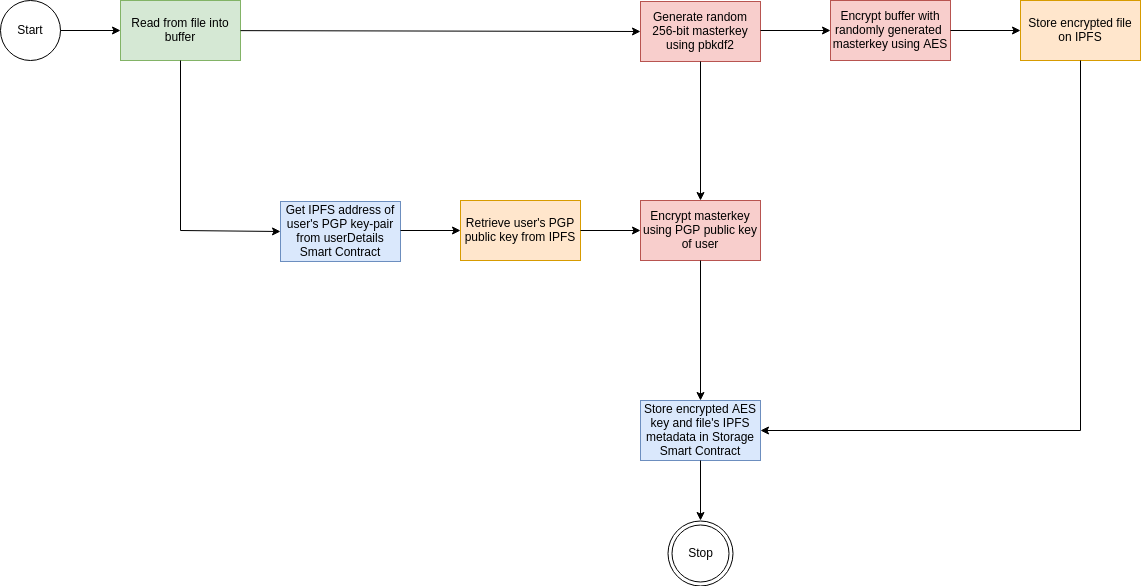
\includegraphics[width=\linewidth]{Images/Encryption.png}
% 	\caption{The Universe}
% 	\label{fig:universe}
% \end{figure}
% \clearpage
% \section{Conclusion}
% \subsection{Objectives Achieved}
% \begin{enumerate}
% 	\item Network deployed on Azure and the statistics for the same. 
% 	\item Implementation of identity management use case which includes the login and the signup 
% 	      module. 
% 	      %\item Writing smart contracts to store necessary details in the blockchain network. 
% 	\item Electronic Health Records Storage on IPFS with encyption. 
% 	\item View the uploaded medical records by the customer. 
% 	\item Policy deployment by an insurance company.
% 	\item User applying for policy and giving access to medical records and premium payment in ethers.
% 	\item Claim settlement based on occurrence of claimable event and claimabled records upload.
% 	\item An interface to view transactions in the blockchain.
% \end{enumerate}
\clearpage